\chapter{要素ごとの寄与の評価}
\label{chap:contribution}
本章では，\ref{sec:sil}節の閉ループシミュレーションを用いて，各要素を除いた場合のラップタイムと完走の可否を比較し，要素ごとの寄与を求める．あわせて，上限速度の段階ごとに制約となる要因を，速度に依存する要求と固定された能力の比較として整理する．本章の主な結果は，実装ソフトウェアをそのまま動かす実装SILで，統一した条件（赤・青コース，上限速度4.0，5.5，7.0\,m/s，実測誤差モデルの知覚雑音，各5シード）により得たものである．過去に同じ処理の流れをPythonで再現した簡易モデルで行った掃引は，合流距離の依存性を示す補足として\ref{sec:merge_result}項に示す．

\section{シミュレーションの妥当性}
\label{sec:sil_validity}
実装SILの妥当性は，次の5つで確認した．第一に，記録した経路生成の出力（目標経路）と自己位置を入力として与えたところ，局所経路計画の出力は記録と0.03〜0.05\,mの範囲で一致した．これは実装が同一であることの確認であり，車両モデルの妥当性を示すものではない．第二に，4章の信号停止の行き過ぎ（実測0.81\,m）を，同定値の範囲内の車両モデル（むだ時間0.27\,s，一次遅れ0.39\,s）を用いた1次元の閉ループ計算で0.73\,mとして再現した（Fig.~\ref{fig:run1012_stop}）．この計算は実装SILではなく，その車両モデルは，実装SILの車両モデル（むだ時間0.06\,s，一次遅れ0.60\,s，Table~\ref{tab:sil_params}）とは別である．また，この車両モデルはむだ時間と一次遅れの組合せを同定値の範囲内で停止の記録に合わせたものであり，同じ記録に対する事後の再現である．第三に，Fig.~\ref{fig:sil_replay}に示すように，R3の隣接車線への移動を，実装の局所経路計画とMPCに自転車モデルを組み合わせ，記録した認識結果を入力とする再生ハーネスの閉ループ（実装SILではない）で再現した．車体のヨーの外乱を与えない場合の横変位は$\pm 0.3$\,mに収まり，記録されたヨーレートから求めた外乱（舵角$-1.6^\circ$相当）を与えると横変位は$-1.1$\,m（実車$-1.4$\,m）となった．外乱の大きさを$-3.0^\circ$相当にすると$-1.9$\,mとなり，横変位は外乱の大きさに応じて変わる．したがってこの再現は，再計画と回避判断の機構が外乱を拡大することを示すものであり，外乱の大きさを独立に予測したものではない．また，記録した認識結果を用いるため，車両が記録軌跡から大きく外れた後の認識入力は実際と整合しない．

第四に，10月12日の走行と同じ構成（MPC，合流距離固定15\,m，2次多項式の平滑化，速度計画の縦加速度6.0\,m/s$^2$，上限速度4.0\,m/s）で赤コースを2周走行させ，実車と比較した（5シード）．2周目のラップタイムは66.9\,sで，実車の68.5\,sに対して2.3\%短い．実車は2.57周（3周目の途中まで）を逸脱なく走行しており，シミュレーションの5本も，すべて2周を完走判定（最大横偏差1.5\,m以内）を満たして走行した．一方，平滑化後の経路に対する横偏差は，95パーセント点が0.93\,m（実車0.57\,m），RMSが0.51\,m（実車0.27\,m）であり，シミュレーションは横偏差を実車の1.6〜1.9倍に見積もる．

第五に，10月12日の走行記録から同定した車両モデルのまま，10月27日のR2とB1の構成を走行させ，日をまたいだ予測を検証した．B1の構成（MPC，青，上限4.5\,m/s，分岐での速度抑制あり）では，シミュレーションの1周目61.5\,s，2周目60.4\,sに対して実車は60.5\,s，59.8\,sで，差は$+1.6$\%，$+1.1$\%（約2\%以内）であった（実車の3周目は制動中に通過したため比較しない）．実車は2.97周を逸脱なく走行しており，シミュレーションの3周も逸脱しなかった．R2の構成（Pure Pursuit法，赤，上限4.0\,m/s，各周に信号停止，青信号までの待ちは3\,sと仮定）では，ラップタイムの平均が75.2\,s（実車73.0\,sに対して3.0\%の差で，3\%の境界上），停止1回あたりの損失が7.3〜8.9\,s（実車4.1〜11.9\,s．シミュレーションは信号ありの周と信号なしの周の差，実車は停止窓による$\Delta T_{\mathrm{stop}}$），停止の行き過ぎが$+0.84$\,mであった．一方，平滑化後の経路に対する横偏差の95パーセント点は，R2でシミュレーション0.35\,mに対して実車0.23\,m（1.5倍），B1で0.17\,mに対して0.33\,m（0.5倍）と，向きが条件によって逆であった．

この横偏差のずれが車両モデルの操舵応答によるものかを，操舵の時定数を0.17\,sから0.44\,sに，ゲインを0.92から1.2に変えて確かめたところ，平滑化後の経路に対する横偏差の95パーセント点は，R2相当で0.35\,m（ゲイン1.2では0.47\,m），B1相当で0.19〜0.20\,m，10月12日相当で0.86〜0.93\,mと，いずれも実車値（0.23，0.33，0.57\,m）に近づかなかった．ここで用いた指標は平滑化後の経路に対する95パーセント点であり，時定数の変更に対してはほぼ不変であった．これに対し，\ref{sec:tracker_result}項の車線中心（真値）に対する最大横偏差（最大値）は，同じ時定数の変更で青コースが1.75〜2.7倍に増える．指標が異なるため両者は矛盾しない．したがって，このずれは操舵応答のモデルでは説明できず，知覚雑音モデルの大きさと系統誤差（B1では小さすぎ，10月12日では大きすぎる），実車の横偏差の基準の取り方の差，およびMPC内部モデルの時定数の違い（10月12日の実車は0.35\,s，SILは0.22\,s）が原因の候補である．

以上から，実装SILは局所経路計画以降の挙動と車両応答に起因する失敗の機構を再現し，実車が逸脱なく走行した区間（10月12日の2.57周，B1の2.97周，R2の3周）ではシミュレーションも逸脱せず，ラップタイムも実車と整合した．ラップタイムの差は，10月12日の構成で2.3\%（実車の68.5\,sには1周あたり約1.3〜1.5\,sの停止損失（4章の$\Delta T_{\mathrm{stop}}$）が含まれ，これを除くと差は約0.2〜0.4\%），日をまたぐ予測でB1が約2\%以内（$+1.6$\%，$+1.1$\%），R2が3.0\%（境界上）であった．一方，横偏差の大きさは条件によって0.5〜1.9倍の範囲で予測できず，その原因は操舵応答のモデルではないと判断した．複数条件でのラップタイムの順位相関は，実車で完走した構成が2つ（R2，R8）にとどまるため算出していない．経路生成そのものは雑音モデルで置き換えているため，学習や重みの違いによる差はシミュレーションでは評価せず，記録した画像に対する開ループの指標で示す．

\begin{figure}[H]
  \centering
  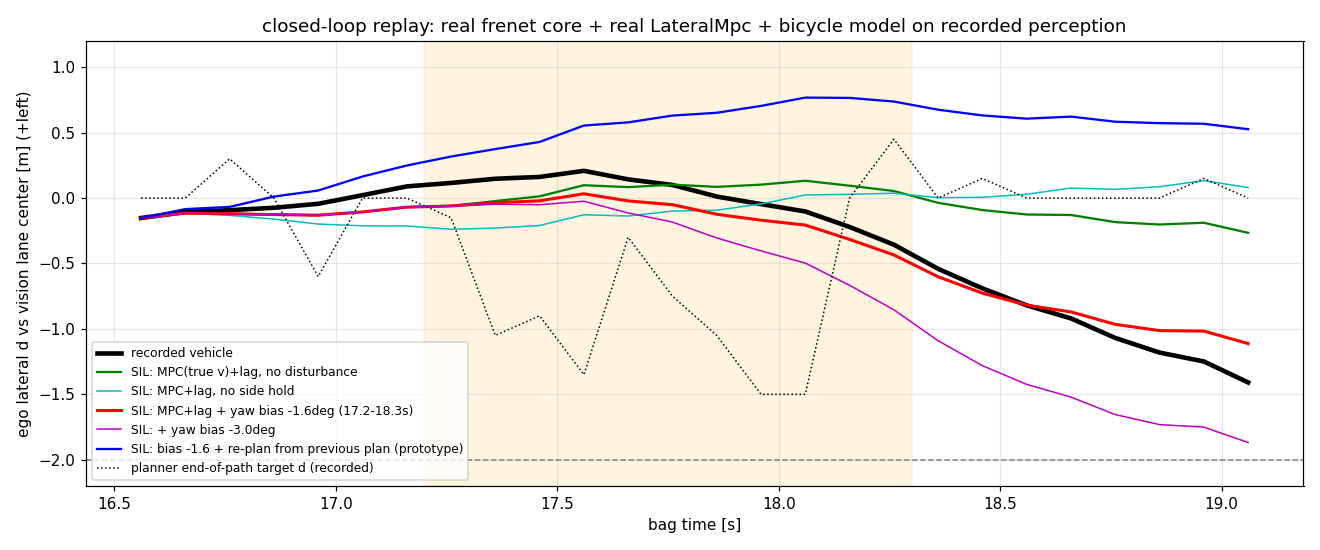
\includegraphics[width=0.85\textwidth]{images/sil_lanechange_replay.png}
  \caption{Closed-loop reproduction of the lane change in R3 with the implemented local planner and MPC and a bicycle model on the recorded perception (a replay harness, not the implemented SIL): lateral position relative to the vision lane center. Lines: recorded vehicle (thick black); simulation without disturbance (MPC with the true speed and lag); simulation without the avoidance-side hold; simulation with a yaw disturbance of $-1.6^\circ$ equivalent steering (17.2--18.3\,s, shaded); the same with $-3.0^\circ$; a prototype with $-1.6^\circ$ that re-plans from the previous plan; and the recorded end-of-path lateral target of the planner (dotted).}
  \label{fig:sil_replay}
\end{figure}

\section{要素ごとのラップタイム}
\label{sec:ablation}
Table~\ref{tab:conditions}に比較する条件の一覧を，Table~\ref{tab:ablation}とFig.~\ref{fig:sil_ablation}に，各要素を除いた条件でのラップタイムと完走の可否を示す．基準構成は，MPC，速度に比例した合流距離（4〜15\,m），3次多項式の平滑化，停止減速度の分離，分岐での速度抑制（青コース，上限4.0\,m/s）である．各走行は2周とし，1周目は発進を含むため2周目のラップタイムを用いる．完走は，2周を走行し，車線中心（真値）に対する最大横偏差が1.5\,m（車線幅の設定値4.0\,mの半分から車両の全幅の上限0.8\,mの半分を引いた1.6\,mを切り下げた値．地図上の車線幅3.65\,mでは同様に約1.4\,m相当）を超えなかった場合と定義する（2.5\,mを超えた時点で打ち切る）．信号停止の成否はこの定義に含めず，\ref{sec:stop_result}項で別に示す（Table~\ref{tab:ablation}の走行は信号停止を含まない）．横偏差は車線中心（真値）に対する値であり，4章の実車の横偏差（経路生成が推定した車線中心に対する値）とは基準が異なる．シミュレーションの周長は赤258.3\,m，青255.3\,mである．

\begin{table}[H]
  \centering
  \caption{Conditions of the component-wise comparison (implemented SIL).}
  \label{tab:conditions}
  \scriptsize
  \begin{lrbox}{\tblbox}\begin{tabular}{L{1.8cm}L{8.2cm}L{4.2cm}}
    \toprule
    条件 & 内容 & 適用 \\
    \midrule
    基準 & MPC，速度に比例した合流距離（4〜15\,m），3次の平滑化，停止減速度の分離，分岐での速度抑制，実測誤差モデル & 赤・青 \\
    A2 & 停止専用の減速度（1.5/4.0\,m/s$^2$）を走行時の縦加速度3.0\,m/s$^2$と共通にする（停止減速度の分離なし） & 赤の信号停止のみ（Table~\ref{tab:ablation}の外，\ref{sec:stop_result}項） \\
    A3 & MPCをPure Pursuit法に置き換える & 赤・青 \\
    A4 & 3次の平滑化を2次に置き換える & 赤・青 \\
    A5 & 合流距離を固定15\,mに置き換える & 赤・青 \\
    A4+A5 & 2次の平滑化かつ固定15\,m（10月12日の実車と同じ組合せ，参考条件） & 赤・青 \\
    A7 & 分岐での速度抑制を外す & 青のみ（赤には分岐がない） \\
    A8 & 理想的な経路生成（雑音なし・認識距離20\,m・平滑化なし） & 赤・青 \\
    A4+A7 & 2次の平滑化かつ分岐での速度抑制を外す（\ref{sec:branch_result}項） & 青のみ \\
    悲観(b)，(c) & 悲観モデルと3次の組合せで，分岐での速度抑制あり(b)，なし(c)（\ref{sec:branch_result}項，\ref{sec:horizon_result}項） & 青，赤は(b)の相当 \\
    6/9\,m切替，4.5/9\,m切替 & 前方6\,m以内にカーブがあるフレームで認識距離を6\,m，4.5\,mに短縮する（\ref{sec:horizon_result}項） & 赤・青 \\
    密な行 & 経路の行を0.5\,m間隔の17行にする（\ref{sec:horizon_result}項） & 青 \\
    9\,m，6\,m打切り & 平滑化の出力を9\,m，6\,mに打ち切る（認識距離9\,m一定，\ref{sec:horizon_result}項） & 青，赤は基準のみ \\
    雑音の倍率 & 実測誤差モデルの雑音を0.5倍，2倍にする（\ref{sec:noise_result}項） & 赤・青 \\
    \bottomrule
  \end{tabular}\end{lrbox}\usebox{\tblbox}
  \tblnote{条件の番号は当初の計画に付けたものを引き継いでおり，番号の振り直しはしない．A1（曲率に基づく速度計画を注視距離による減速に置き換える）とA6（回避側の保持を外す）は当初の計画にあった条件であるが，本論文では実施していない（欠番）．}
\end{table}

各条件は5シードであるため，完走率のWilsonの方法による95\%信頼区間は5/5で[0.57, 1.00]，3/5で[0.23, 0.88]，1/5で[0.04, 0.62]，0/5で[0.00, 0.43]であり，区間が重ならないのは0/5と5/5の組だけである．区間の重なりは保守的な目安にすぎないため，Fisherの正確検定（両側）のp値を併記すると，5/5対0/5で$p\approx 0.008$，5/5対1/5で$p\approx 0.048$，5/5対3/5で$p\approx 0.44$である．条件数が多く多重比較の補正は行っていないため，$p\approx 0.048$も区別できる差としては扱わない．したがって本章で完走の可否の差として述べるのは，5/5と0/5のように全試行で結果が分かれた場合に限り，3/5や1/5のような中間の値は傾向として扱い，その差は完走率ではなく最大横偏差（連続量）で述べる．ラップタイムは同じ条件ではシード間の標準偏差が0.0〜0.44\,s（完走した試行の標本標準偏差）であり，その2倍（約0.9\,s）を超えない差は条件間の差として扱わない．基準との2周目ラップタイムの差をWelchのt検定（両側）で確かめると，A7（青）は5.5\,m/sで$-3.19$\,s（$p=1\times 10^{-6}$），7.0\,m/sで$-4.31$\,s（$p=2\times 10^{-6}$），A5（赤の7.0\,m/s）は$+1.05$\,s（$p=4\times 10^{-5}$）と有意である．0.2〜0.5\,sの小さな差には，A4の青5.5\,m/s（$-0.22$\,s，$p=2\times 10^{-4}$）やPure Pursuit法の青5.5\,m/s（$+0.23$\,s，$p=4\times 10^{-4}$）のようにp値が小さいものと，A4の青7.0\,m/s（$-0.52$\,s，$p=0.008$）やPure Pursuit法の赤7.0\,m/s（$-0.30$\,s，$p=0.018$）のように大きいものがある．比較数が多い（各表約20セル）ため，Bonferroniの補正（有意水準$0.05/20$）を参考値として用いると，後者は有意でない．また，4.0\,m/sのセルは上限速度でラップタイムが決まり標準偏差がほぼ0であるため，p値は不安定である．なお，信頼区間と検定は5シードの標本の不確かさだけを表し，車両モデルと雑音モデルの不確かさ（実車との比較で横偏差が0.5〜1.9倍ずれた，\ref{sec:sil_validity}節）を含まない．完走の判定は横偏差の閾値で行うため，後者の影響の方が支配的である．

\begin{table}[H]
  \centering
  \caption{Lap time of the second lap (mean of completed runs), number of completed runs, and mean maximum lateral deviation from the true lane center with each component removed (implemented SIL, 5 seeds per cell).}
  \label{tab:ablation}
  \scriptsize
  \begin{lrbox}{\tblbox}\begin{tabular}{L{2.5cm}L{1.6cm}L{1.6cm}L{1.6cm}L{1.6cm}L{1.6cm}L{1.6cm}}
    \toprule
    & \multicolumn{3}{c}{赤コース} & \multicolumn{3}{c}{青コース} \\
    条件 & 4.0\,m/s & 5.5\,m/s & 7.0\,m/s & 4.0\,m/s & 5.5\,m/s & 7.0\,m/s \\
    & s / 完走 / m & s / 完走 / m & s / 完走 / m & s / 完走 / m & s / 完走 / m & s / 完走 / m \\
    \midrule
    基準 & 66.9 / 5 / 0.12 & 48.7 / 5 / 0.16 & 39.1 / 5 / 0.19 & 66.2 / 5 / 0.16 & 52.7 / 5 / 0.20 & 46.1 / 5 / 0.20 \\
    A3 Pure Pursuit法 & 66.9 / 5 / 0.41 & 48.7 / 5 / 0.54 & 38.8 / 5 / 0.81 & 66.1 / 5 / 0.81 & 52.9 / 5 / 0.80 & 46.1 / 5 / 0.87 \\
    A4 2次多項式の平滑化 & 66.9 / 5 / 0.11 & 48.7 / 5 / 0.13 & 38.8 / 5 / 0.17 & 66.1 / 5 / 0.48 & 52.5 / 5 / 0.60 & 45.6 / 5 / 0.44 \\
    A5 合流距離固定15\,m & 66.9 / 1 / 1.66 & 48.8 / 3 / 1.55 & 40.2 / 3 / 1.40 & -- / 0 / 2.49 & -- / 0 / 2.50 & -- / 0 / 2.47 \\
    A4+A5 2次かつ固定15\,m & 66.9 / 5 / 1.11 & 48.7 / 5 / 1.00 & 38.3 / 5 / 0.92 & -- / 0 / 1.70 & -- / 0 / 1.82 & -- / 0 / 1.80 \\
    A7 分岐での速度抑制なし & -- & -- & -- & 66.2 / 5 / 0.19 & 49.5 / 5 / 0.18 & 41.8 / 5 / 0.28 \\
    A8 理想的な経路生成 & 66.9 / 5 / 0.12 & 48.7 / 5 / 0.10 & 38.8 / 5 / 0.12 & 66.2 / 5 / 0.39 & 52.7 / 5 / 0.33 & 45.6 / 5 / 0.33 \\
    \bottomrule
  \end{tabular}\end{lrbox}\usebox{\tblbox}
  \tblnote{A5の青コースの最大横偏差2.47〜2.50\,mは，2.5\,mで打ち切った走行の値の平均である．A7は青コースのみで行った（赤コースには分岐がない）．}
\end{table}

\begin{figure}[H]
  \centering
  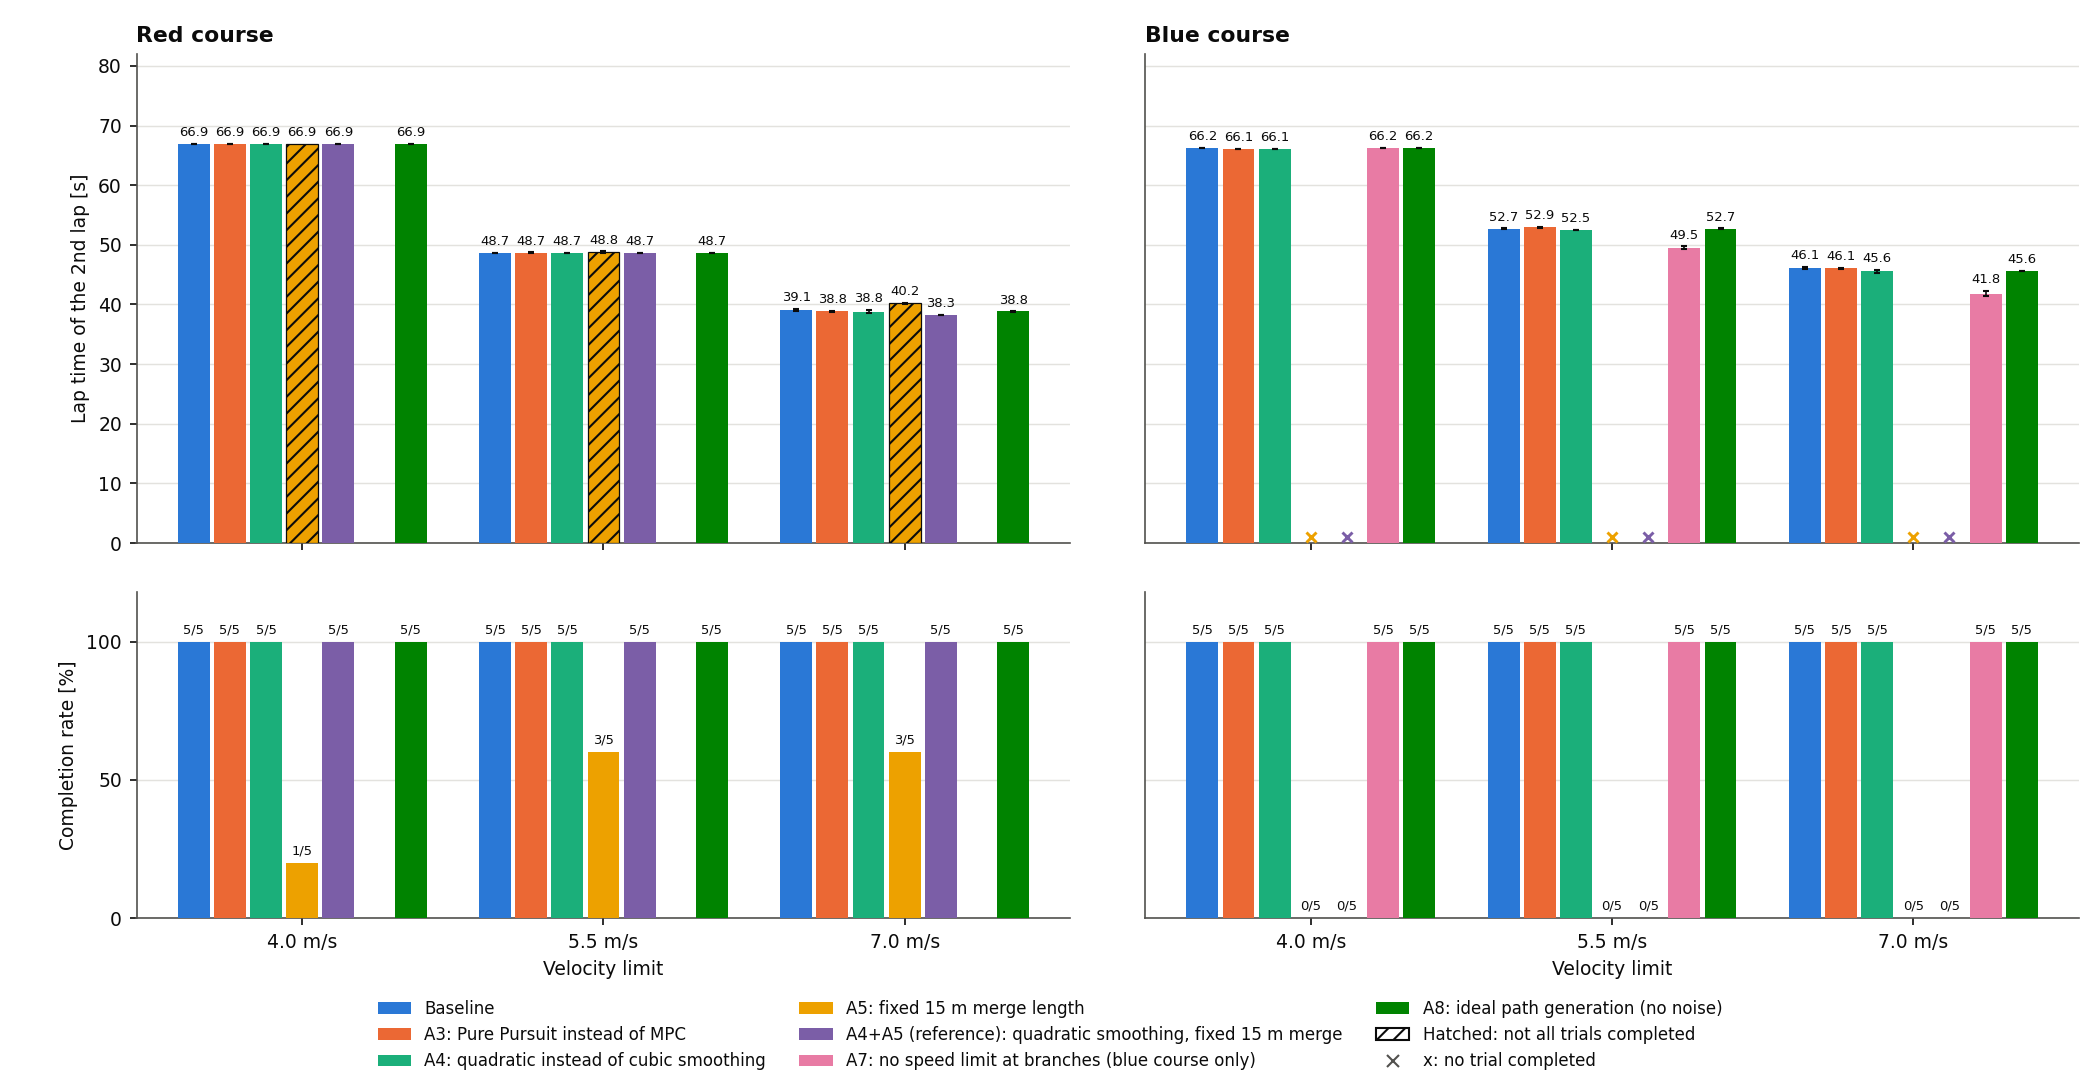
\includegraphics[width=0.98\textwidth]{images/sil_ablation.png}
  \caption{Second-lap time (top) and completion rate (bottom) for each condition and upper speed limit in the implemented SIL (left: red course, right: blue course, 5 seeds). A4+A5 (quadratic smoothing and fixed 15\,m merge length) is a reference condition. A7 is shown for the blue course only because the red course has no branch. Hatched bars: not all trials completed; crosses: no trial completed.}
  \label{fig:sil_ablation}
\end{figure}

完走した条件では，上限速度4.0\,m/sのラップタイムは66.9\,s（赤）と66.1〜66.2\,s（青）で差がなく，4章の内訳と同じく上限速度がラップタイムを決めている．条件間の差は，完走の可否と横偏差，および上限速度5.5\,m/s以上のラップタイムに現れる．ただし，赤コース7.0\,m/sでは基準の39.1\,sがA3，A4，A8の38.8\,sより0.3\,s，A4+A5の38.3\,sより0.9\,s遅い．0.3\,sの差はBonferroniの補正後は有意でなく，0.9\,sの差（A4+A5，$p=4\times 10^{-4}$）は有意であるがシード間の標準偏差の2倍以内であり，A4+A5は参考条件であるため，要素の寄与としては扱わない．基準構成は赤・青とも7.0\,m/sまで5本すべてが完走し，最大横偏差は0.12〜0.20\,mであった．この結果は，カーブで認識距離を6\,mに短縮した条件でも変わらなかった（\ref{sec:horizon_result}項）．以下に要素ごとの結果を述べる．

\subsection{局所経路計画の合流距離}
\label{sec:merge_result}
完走の可否を左右した要素は合流距離である．合流距離を15\,mに固定した条件（A5）では，青コースは全速度で5本すべてが失敗し（最大横偏差2.5\,m，打ち切り），赤コースの完走は4.0，5.5，7.0\,m/sで5本中1，3，3本であった．赤コースの完走数は中間の値であるため，基準（5/5）との差は完走率ではなく最大横偏差で述べる．最大横偏差の平均（最悪）は，基準が0.12〜0.19\,mであるのに対し，A5は1.40〜1.66\,m（1.58〜2.00\,m）である（Table~\ref{tab:ablation}）．合流距離を車速に比例させ横加速度の上限で下限を与えた基準構成では，赤・青とも全速度で5本すべてが完走した．

ただし，この結果は平滑化の次数と組み合わさって変わる．2次多項式の平滑化と固定15\,mを組み合わせた条件（A4+A5）では，赤コースは全速度で5本すべてが完走し（Table~\ref{tab:ablation}の最大横偏差0.92〜1.11\,m），青コースは完走しなかった．10月12日の実車走行はこの組合せ（2次，固定15\,m）で赤コースを完走しており，シミュレーションの結果と矛盾しない．

3次多項式の平滑化と固定15\,mの組合せで赤コースの最大横偏差が大きくなる機構を，記録したトレースと介入実験で調べた（Fig.~\ref{fig:sil_merge_mech}）．上限4.0\,m/sのA5の既存5本では，最大横偏差は5本中4本で半径約9.5\,mのカーブ（$s=79$〜$98$\,m）の出口（$s\approx 99$〜$102$\,m）に生じ（残りの1本はシード3の$s=186$\,m，最大1.23\,mで完走），$s\approx 70$\,mから約25\,mをかけて1.6〜2.0\,mまで緩やかにカーブの外側へ成長する．5.5，7.0\,m/sでは，最大の位置はこのカーブの出口に集まらない．舵角の指令値は最大$7.2^\circ$（A5のシード2）で飽和しておらず，経路の折れも完走する基準構成と同程度である．この条件では，平滑化後の経路の点のある範囲（認識距離，約9\,m）の外側にある$x=15$\,mでの，真の車線中心に対する誤差の絶対値の平均が3次で3.8\,m，2次で1.8\,mと約2倍であった．そこで，合流の終点がこの外挿部に入ることが原因であるという仮説を，外挿誤差を人為的に変える介入で検証した．雑音のない真値の点を9\,m以遠に加えて$x=15$\,mの外挿誤差を0.6〜0.8\,mに減らした介入（実装には存在しない検証用の条件）では，完走が0/5に悪化し，この仮説は支持されなかった．また，固定10\,mの条件でも$x=15$\,mの誤差は3.8\,mと固定15\,mと同じであるが完走するため，外挿誤差の大きさは完走と対応しない．

一方，合流距離の設定値と平滑化後の経路の長さの小さい方（以下，合流の実効距離）を変えた介入では，Table~\ref{tab:merge_intervention}に示すように，最大横偏差の平均（最悪）は，実効距離が約9\,mと10\,mの条件で0.47〜0.59\,m（0.65〜0.79\,m），約12\,mと15\,mの3次の条件で1.48〜1.76\,m（1.71〜2.22\,m）と2群に分かれ，前者は5本すべてが完走した（赤，4.0と5.5\,m/s，各5シード）．なお，真値の点を加えた15\,mの条件は2.30〜2.43\,m（最悪2.44〜2.51\,m），2次の15\,mの条件は1.01〜1.15\,mで，どちらの群にも入らない．完走数の1/5，3/5と5/5は規則上区別できないため，群の差は最大横偏差（最悪値を含む）で述べ，完走の差として区別できるのは真値の点を加えた条件（0/5）と実効距離10\,m以下の条件（5/5）だけである．実効距離を10\,m以下にした条件では，試した範囲（赤コース，4.0と5.5\,m/s）で，3次（固定10\,m，出力の9\,m打ち切り）でも2次（A4，速度に比例した合流4〜7\,m）でも完走した．

実効距離が長い3次の条件で最大横偏差が大きくなる機構としては，局所経路が毎周期，計測した自己位置から再計算されるため，長い合流では追従制御の補正が次の周期の経路に打ち消され，車両がカーブの外側へ膨らむことが考えられる．3次の条件では最大横偏差の向きはすべてカーブの外側で，カーブ中の符号付きの平均横偏差は固定15\,mで$-0.58$\,m，固定10\,mで$-0.21$\,mである．ただしこれは因果を確かめたものではなく，局所経路の$x=5$\,mでの誤差（Table~\ref{tab:merge_intervention}，固定15\,mで0.58\,m，固定10\,mで0.14\,m）と最大横偏差が同じ向きに変わるという相関に基づく説明である．この説明では，次の2点が未解明である．第一に，同じ実効距離15\,mで，2次の平滑化は完走し（最大横偏差1.15\,m，Table~\ref{tab:merge_intervention}の値），3次は完走しない（1.76\,m）．2次ではカーブ中の符号付きの平均横偏差が内側へ$+0.08$\,mである．また，$x=15$\,mでの外側への偏り（符号付きの平均）は2次で1.4\,m，3次で0.6\,mと2次の方が大きく，絶対値の平均（1.8\,m対3.8\,m）とは大小が逆である．第二に，真値の点を加えて外挿誤差を小さくした条件（2.30\,m，0/5）が，かえって悪化する．これらは「長い合流ほど補正が打ち消される」だけでは説明できず，本研究では原因を特定できていない．

なお，青コースのA4+A5（2次・固定15\,m）の失敗は，赤コースのA5とは異なる．全15走行（3速度，各5シード）で最大横偏差はカーブの内側に生じ（赤コースのA5は外側），位置は交差点カーブ内（$s=174$〜176\,m）が7走行，分岐カーブの出口後の緩いカーブ（$s=140$〜143\,m）が8走行で，最大横偏差は1.62〜1.96\,mであった．この機構は未解明である．

\begin{figure}[H]
  \centering
  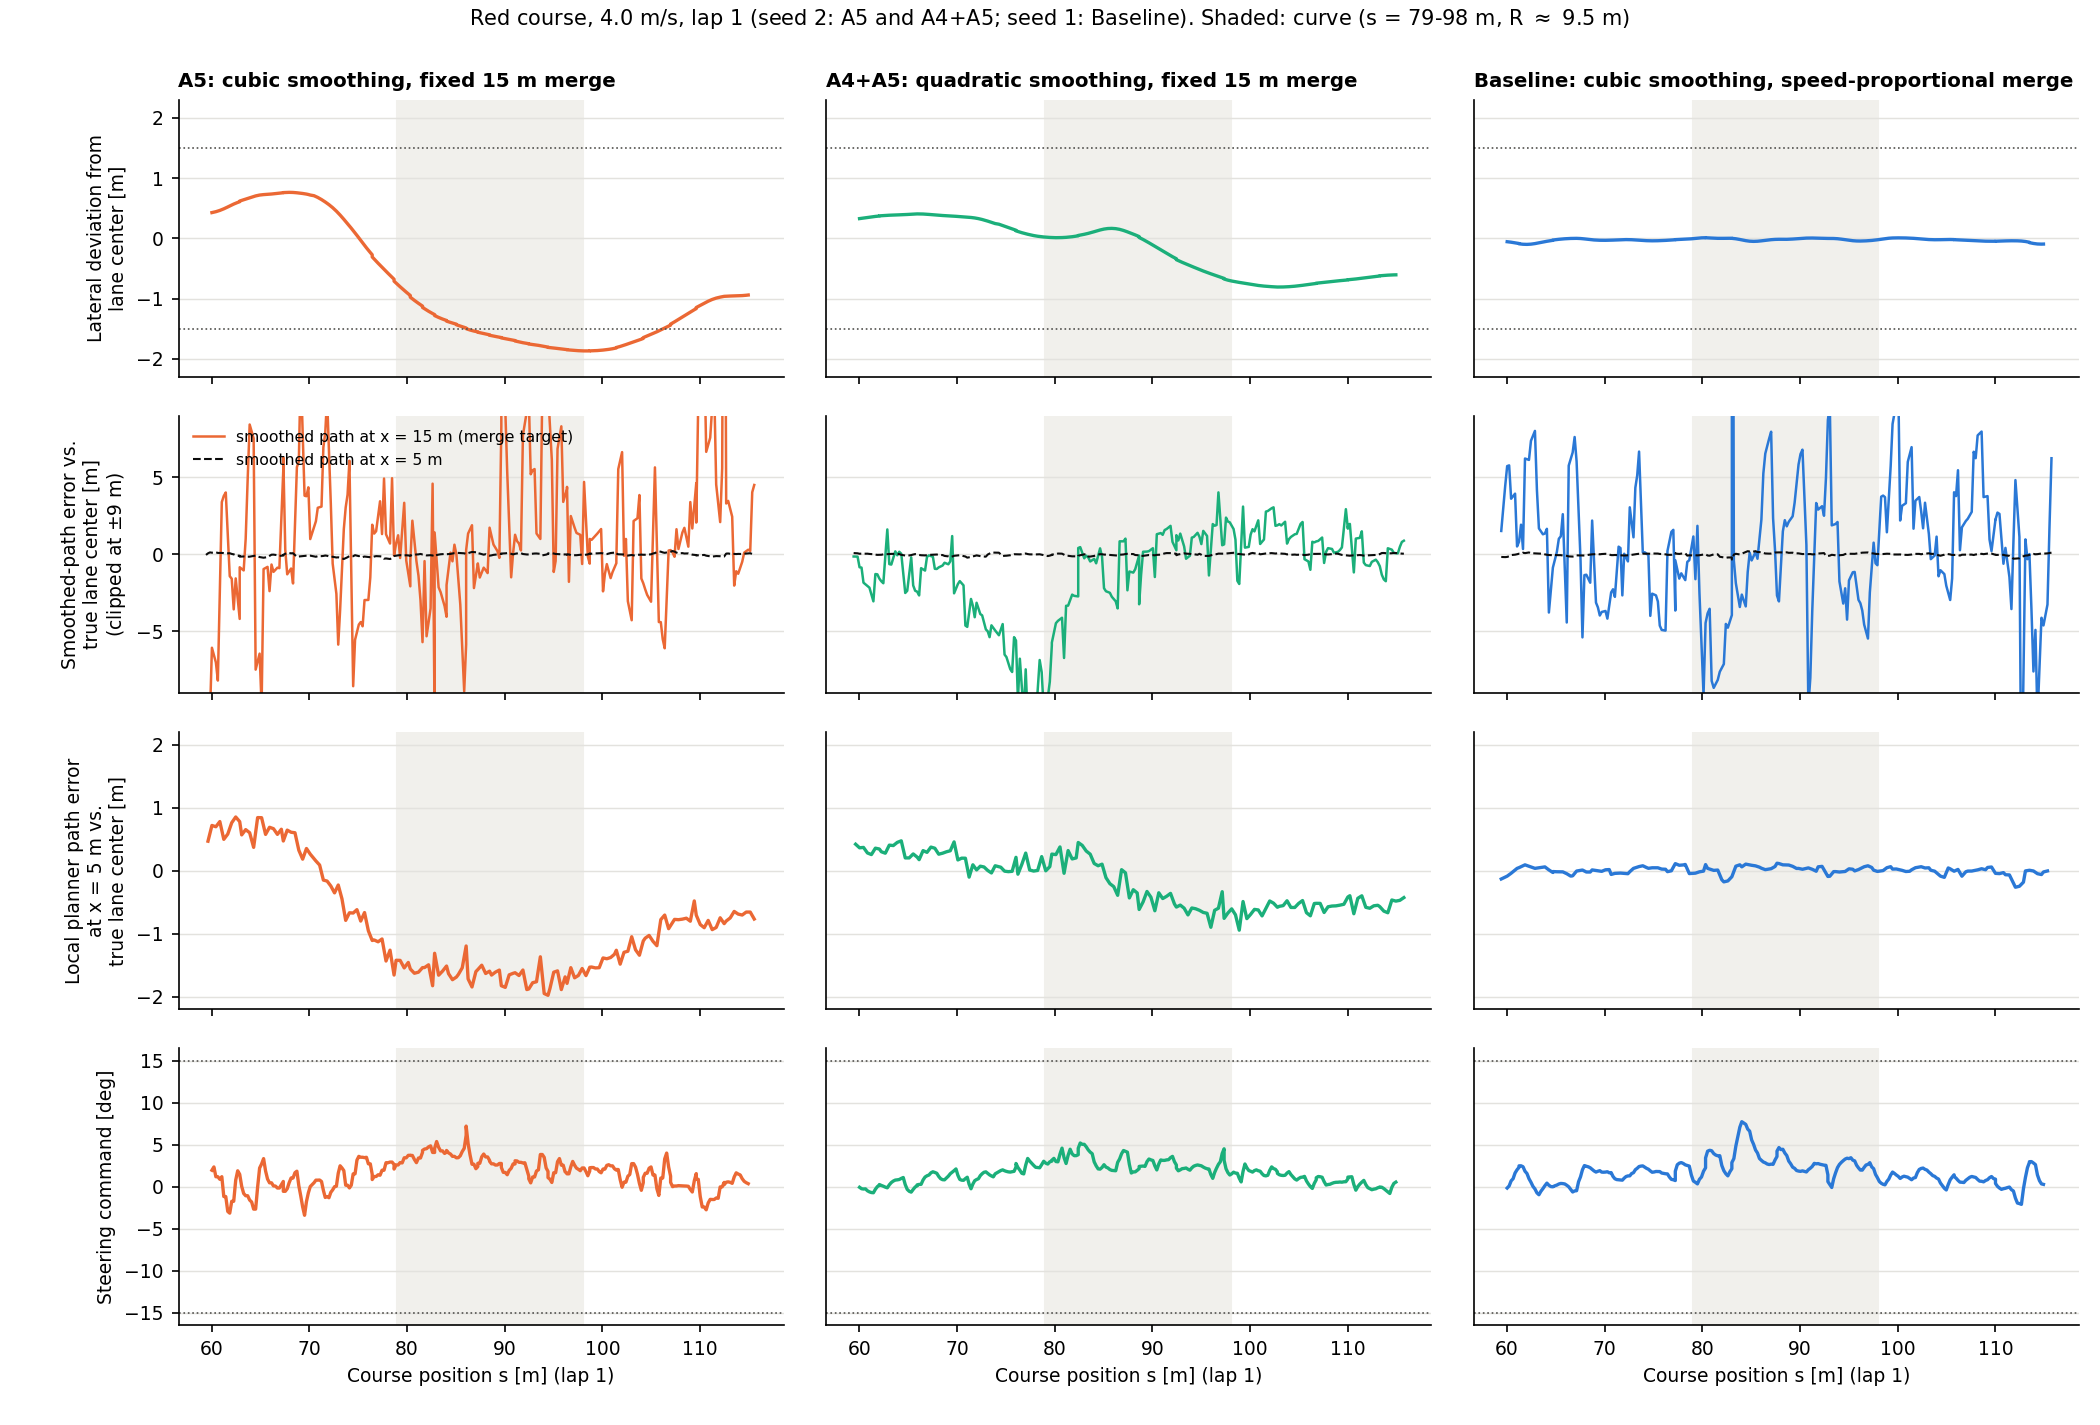
\includegraphics[width=0.95\textwidth]{images/sil_merge_mechanism.png}
  \caption{Failure with a fixed merge length of 15\,m and cubic smoothing on the red course (implemented SIL, 4.0\,m/s, lap 1; seed 2 for A5 and A4+A5, seed 1 for the baseline), compared with quadratic smoothing and with the velocity-proportional merge length. From top: lateral deviation from the lane center; error of the smoothed path at $x=15$\,m (colored) and at $x=5$\,m (dashed) with respect to the true lane center, clipped at $\pm 9$\,m; error of the local path at $x=5$\,m; steering command. The second panel shows the extrapolation error that was hypothesized as the cause; this hypothesis was not supported by the intervention experiments in the text. The traces are from reruns with path recording under the same conditions and seeds.}
  \label{fig:sil_merge_mech}
\end{figure}

\begin{table}[H]
  \centering
  \caption{Interventions on the failure with a fixed merge length of 15\,m on the red course (implemented SIL, MPC, measured error model of the path generation, 5 seeds each). The effective merge length is the smaller of the merge setting and the smoothed path length. The condition with true far points is an oracle input that does not exist in the implementation. The first and last rows are reruns of A5 and A4+A5 of Table~\ref{tab:ablation} and differ from the values in that table.}
  \label{tab:merge_intervention}
  \scriptsize
  \begin{lrbox}{\tblbox}\begin{tabular}{L{4.4cm}ccccccc}
    \toprule
    条件 & 実効距離 & \multicolumn{4}{c}{上限速度 [m/s]} & \multicolumn{2}{c}{経路誤差 [m]} \\
    \cmidrule(lr){3-6}\cmidrule(lr){7-8}
    & [m] & \multicolumn{2}{c}{完走} & \multicolumn{2}{c}{最大横偏差 [m]} & $x=15$ & 局所 $x=5$ \\
    \cmidrule(lr){3-4}\cmidrule(lr){5-6}
    & & 4.0 & 5.5 & 4.0 & 5.5 & & \\
    \midrule
    3次・固定15\,m（Table~\ref{tab:ablation}のA5と同条件の再実行） & 15 & 1/5 & 3/5 & 1.76 (1.93) & 1.54 (2.22) & 3.8 & 0.58 \\
    3次・固定10\,m & 10 & 5/5 & 5/5 & 0.59 (0.67) & 0.53 (0.65) & 3.8 & 0.14 \\
    3次・固定15\,m・出力12\,m打切り & 約12 & 2/5 & 3/5 & 1.48 (1.71) & 1.56 (2.14) & --- & 0.41 \\
    3次・固定15\,m・出力9\,m打切り & 約9 & 5/5 & 5/5 & 0.56 (0.79) & 0.47 (0.72) & --- & 0.10 \\
    3次・固定15\,m・真値の点を追加 & 15 & 0/5 & 0/5 & 2.30 (2.44) & 2.43 (2.51) & 0.6 & 0.81 \\
    2次・固定15\,m（A4+A5と同条件の再実行） & 15 & 5/5 & 5/5 & 1.15 (1.22) & 1.01 (1.12) & 1.8 & 0.31 \\
    \bottomrule
  \end{tabular}\end{lrbox}\usebox{\tblbox}
  \tblnote{最大横偏差は車線中心（真値）に対する値の5シード平均（括弧内は最悪値）．経路誤差は4.0\,m/sの値で，前方15\,m以内にカーブがあるフレーム（カーブ内を含む）で真の車線中心に対して測った絶対値の平均．$x=15$\,mは平滑化後の経路，局所 $x=5$\,mは追従制御が追う局所経路の値．実効距離の約9，約12\,mは平均8.9，11.9\,m．「真値の点を追加」は9\,m以遠に雑音のない真値の点を加えた条件．第1行と最終行は，Table~\ref{tab:ablation}のA5，A4+A5と同じ条件を再実行した別の走行であり，その値（A5の赤は1.66，1.55\,m，A4+A5は1.11，1.00\,m）とは異なる．}
\end{table}

Fig.~\ref{fig:sil_merge}に，補足として簡易モデルによる合流距離5〜15\,mの掃引を示す．合流距離が長いほど最大横偏差は大きく，15\,mでは完走の判定である1.5\,mに達する．

\begin{figure}[H]
  \centering
  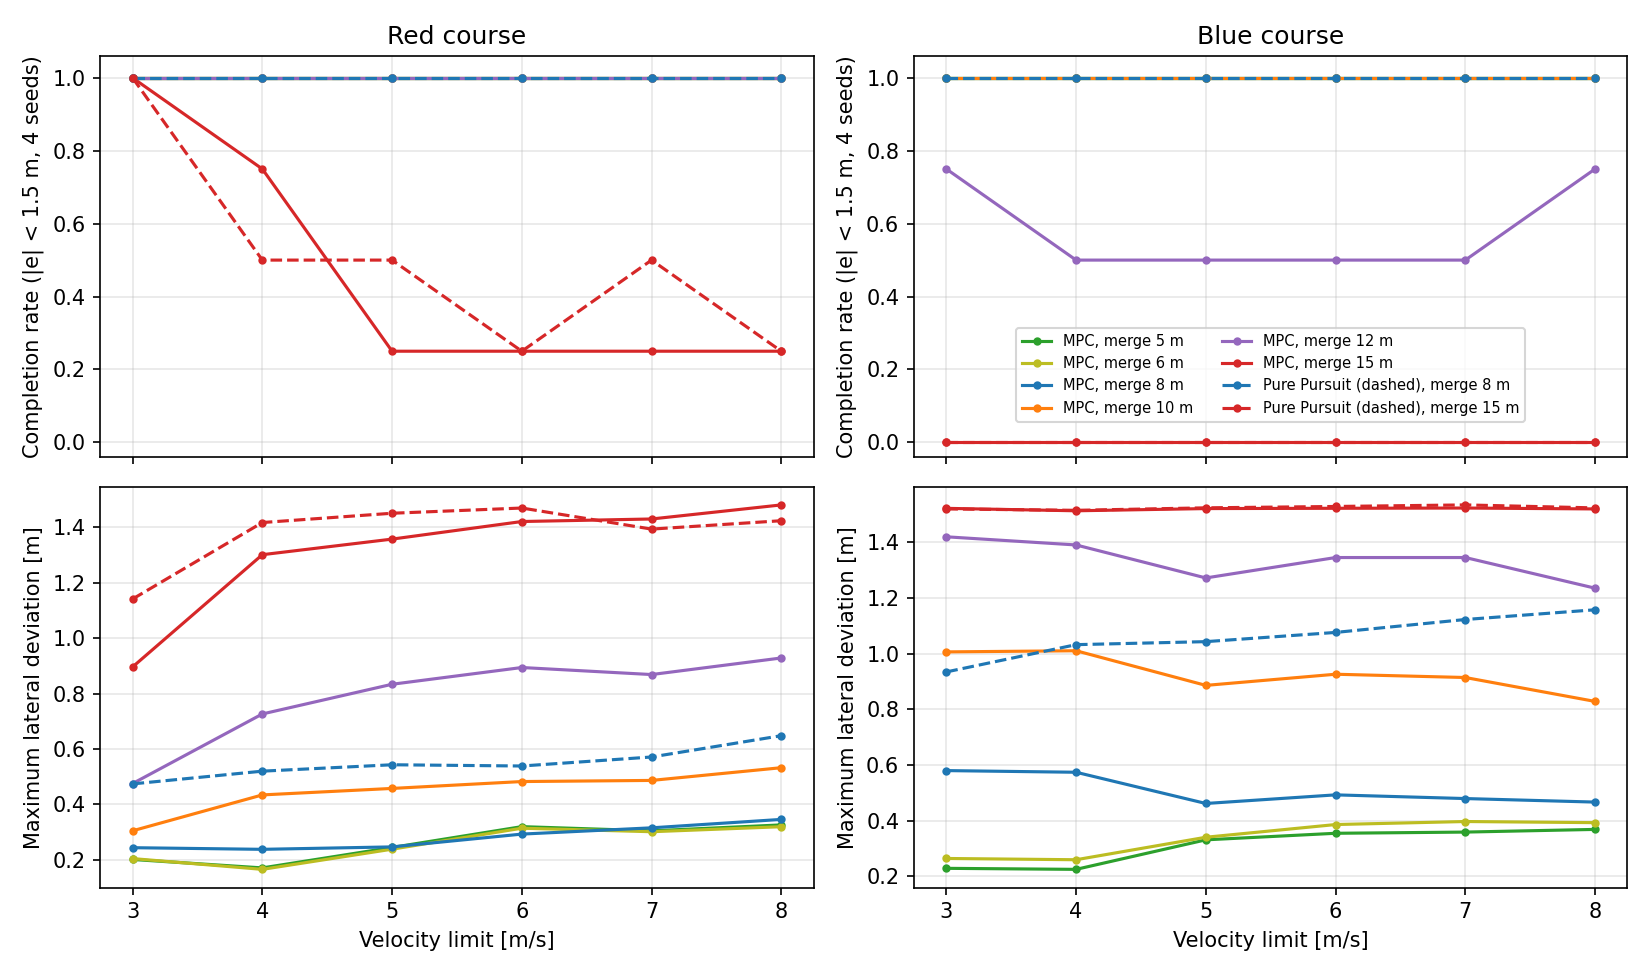
\includegraphics[width=0.85\textwidth]{images/sil_merge_sweep.png}
  \caption{Completion rate (top) and maximum lateral deviation (bottom) versus the upper speed limit for fixed merge lengths of 5 to 15\,m in the simplified closed-loop model (left: red course, right: blue course, 4 seeds). MPC is drawn with solid lines and Pure Pursuit with dashed lines (merge lengths of 8\,m and 15\,m only). Runs are aborted when the deviation exceeds 1.5\,m.}
  \label{fig:sil_merge}
\end{figure}

\subsection{経路追従制御}
\label{sec:tracker_result}
MPCをPure Pursuit法に置き換えた条件（A3）では，完走の可否は変わらず（30本すべて完走），ラップタイムの差も0.3\,s以内であった．一方，最大横偏差は赤コースで0.12〜0.19\,mから0.41〜0.81\,m，青コースで0.16〜0.20\,mから0.80〜0.87\,mに増え，同一シード対の比の平均は3.5〜5.1（シードごとの比は2.7〜6.0）であり，MPCは横偏差を1/3.5〜1/5（シードごとには1/2.7〜1/6）にする．すなわち，追従制御の寄与はラップタイムではなく横偏差の大きさに現れる．

操舵の時定数を手動走行の同定値0.17\,sから自律走行中の当てはめ値0.44\,sに変えた場合（青コース，基準構成），ラップタイムの変化は0.1\,s，完走は5本すべてのままで，最大横偏差（車線中心（真値）に対する最大値の平均）は4.0\,m/sで0.16\,mから0.43\,m（2.7倍），5.5\,m/sで0.20\,mから0.35\,m（1.75倍）に増えた．一方，同じ走行の横偏差の95パーセント点は，0.09\,mから0.12\,m，0.11\,mから0.17\,mへの増加（1.3〜1.5倍）にとどまる．時定数の不確かさは最大横偏差の見積もりに影響するが，完走とラップタイムの結論は変わらない．

\subsection{経路の平滑化}
\label{sec:smoother_result}
3次多項式の平滑化を2次に戻した条件（A4）のラップタイムは，3次との差が赤コースの4.0，5.5，7.0\,m/sで0.0，0.0，0.3\,s，青コースで0.1，0.2，0.5\,sであり，いずれもシード間の標準偏差の2倍（約0.9\,s）以内であるため，差としては扱わない．赤コースの横偏差はほぼ同じであった．青コースでは3次の方が最大横偏差を0.44〜0.60\,mから0.16〜0.20\,mに減らした．この差を3次が曲率を早く捉えるためとは言えない．\ref{sec:horizon_result}項の記録では，3次の曲率比（平滑化後の経路から求めた曲率を走行した曲率で割った値）は2.5\,m先で0.79，4\,m先で0.53と2次（0.49，0.47）より高いが，6\,m先では0.19と2次（0.41）より小さい．青コースで3次の最大横偏差が小さい機構は，本研究では特定できていない．

\subsection{分岐での速度抑制}
\label{sec:branch_result}
青コースで分岐での速度抑制を外した条件（A7）では，5本すべてが完走し，ラップタイムは基準に対して5.5\,m/sで3.2\,s（6.1\%），7.0\,m/sで4.3\,s（9.3\%）短縮した（Welchの検定でどちらも$p<10^{-5}$．4.0\,m/sでは基準と同じ66.2\,s）．この結果は平滑化や経路生成の条件を変えても変わらず，2次の平滑化（A4+A7），および悲観モデル（実測誤差に加え，近傍の接線からの偏差に$1/(1+(x/8)^2)$を掛けて遠方の曲りを減らすモデル，\ref{sec:sil}節）と3次の組合せのいずれも，抑制を外して7.0\,m/sまで5本すべてが完走し（7.0\,m/sの最大横偏差0.3〜0.6\,m），ラップタイムは抑制ありに対して5.5\,m/sで$-3.2$〜$-4.1$\,s，7.0\,m/sで$-4.3$〜$-5.8$\,s短縮した．実車のB1（上限4.5\,m/s，抑制値4.0\,m/s）で抑制が生んだ時間差は1周あたり1.1\,s（2.97周で3.2\,s，4章）であり，上限速度と抑制値の差が小さいため，これらより小さい．

代償として，交差点カーブ（半径約4.6\,m）の最大横加速度が増える．抑制あり（3次・実測誤差モデル）では，4.0〜9.0\,m/sのどの上限速度でも平均2.5〜2.9\,m/s$^2$にとどまる（7.0\,m/sでは1シードが4.5\,m/s$^2$）が，抑制なしのA7では，Table~\ref{tab:branch_ay}に示すように5.5\,m/s以上で速度計画の設計上限$a_{y,\max}=3.0$\,m/s$^2$を超え（5.0\,m/sで2.9，5.5\,m/sで3.4，7.0\,m/sで4.0\,m/s$^2$），7.5\,m/s以上ではいずれかのシードが摩擦限界の6.0\,m/s$^2$に達し，9.0\,m/sでは完走が3/5になる．2次の平滑化（A4+A7）と悲観モデルでは，5.5\,m/sで4.7\,m/s$^2$，7.0\,m/sで6.0\,m/s$^2$（2次）と5.8\,m/s$^2$（悲観モデル）に達し，2次の7.0\,m/sは摩擦限界に張り付く．したがって，分岐での速度抑制は完走には不要であるが，3次の平滑化と実測誤差モデルでは交差点カーブの横加速度を設計上限内に保つ機能を持ち，抑制なしでは設計上限を5.5\,m/s以上で超え，完走は摩擦限界までの余裕で保たれているにすぎない．ただし，抑制ありの基準構成でも，周回全体の最大横加速度（平均）は赤の5.5\,m/sで3.1，7.0\,m/sで4.4，9.0\,m/sで5.8，青の7.0\,m/sで4.3\,m/s$^2$と設計上限を超える（Fig.~\ref{fig:sil_horizon6}）．なお，4.0\,m/sでは上限速度と抑制値が同じであり，A7と基準は同じ構成であるが，Table~\ref{tab:branch_ay}の値は2.8と2.6\,m/s$^2$，最大横偏差は0.19と0.16\,mと異なり，この差はSILの非決定性の大きさを示す．Fig.~\ref{fig:sil_branch}に，統一条件での上限速度5.5，7.0\,m/sの速度を示す．網掛けはSILが記録した経路選択の指示が直進以外の区間で，速度上限が有効だった区間と（DDS遅延約0.05\,sの差で）一致する．抑制なし（赤）は分岐カーブと交差点カーブの直前まで上限に近い速度で進入し，曲率から決まる上限（破線）に沿って減速するのに対し，抑制あり（緑）は指示区間の大部分を4\,m/s前後で走行する．ただし，指示は$s=108.6$\,mでonになり179.7\,mでoffになる間の$s\approx 128.5$〜130\,mと153〜154.8\,mの2か所で約0.4\,sだけ直進に戻り，そこで上限が解除されて速度指令が上限速度に戻るため，車両の速度応答（一次遅れ0.60\,s）と0.3\,s先の参照により，隙間の終端から約3.5\,m先で4.5〜4.9\,m/sのピークになり，4.0\,m/sに戻るまで約8\,mかかる（5.5\,m/sで$4.82\pm 0.07$，$4.53\pm 0.14$，7.0\,m/sで$4.84\pm 0.30$，$4.59\pm 0.12$）．入口（$s=108.5$\,m）は上限速度からの減速の途中である．この隙間はSILの指示生成（旋回の完了で直進を出し，次のノードが20\,m以内に入るまで直進）によるもので，実車のトポロジカルマップの指示で同じ隙間が生じるかは確認していない．隙間がなければ，抑制ありの速度は4.0\,m/s付近に保たれ，A7のラップ短縮は今回の値より少し大きく出る可能性がある．

\begin{table}[H]
  \centering
  \caption{Maximum lateral acceleration in the section of the T-junction curve ($s=169$--$184$\,m, $R\approx 4.6$\,m) of the blue course versus the upper speed limit, without (A7) and with (baseline) the branch speed reduction (implemented SIL, 5 seeds; mean $\pm$ SD (maximum) in m/s$^2$). The design limit of the velocity planner is 3.0\,m/s$^2$ and the grip limit is 6.0\,m/s$^2$. At 4.0\,m/s the two columns are the same configuration, so their difference shows the non-determinism of the simulation.}
  \label{tab:branch_ay}
  \small
  \begin{tabular}{rccc}
    \toprule
    上限速度 [m/s] & A7（抑制なし） & 完走（A7） & 基準（抑制あり） \\
    \midrule
    4.0 & 2.8$\pm$0.2 (3.0) & 5/5 & 2.6$\pm$0.2 (2.9) \\
    5.0 & 2.9$\pm$0.2 (3.1) & 5/5 & 2.7$\pm$0.1 (2.9) \\
    5.5 & 3.4$\pm$0.3 (3.8) & 5/5 & 2.6$\pm$0.2 (2.9) \\
    6.0 & 3.8$\pm$0.3 (4.2) & 5/5 & 2.6$\pm$0.3 (3.0) \\
    6.5 & 3.9$\pm$0.3 (4.2) & 5/5 & 2.6$\pm$0.1 (2.7) \\
    7.0 & 4.0$\pm$0.4 (4.4) & 5/5 & 2.9$\pm$0.9 (4.5) \\
    7.5 & 4.9$\pm$0.8 (6.0) & 5/5 & 2.6$\pm$0.2 (2.8) \\
    8.0 & 5.5$\pm$0.7 (6.0) & 5/5 & 2.5$\pm$0.2 (2.8) \\
    8.5 & 5.6$\pm$0.6 (6.0) & 5/5 & 2.5$\pm$0.2 (2.8) \\
    9.0 & 6.0$\pm$0.0 (6.0) & 3/5 & 2.6$\pm$0.1 (2.7) \\
    \bottomrule
  \end{tabular}
\end{table}

\begin{figure}[H]
  \centering
  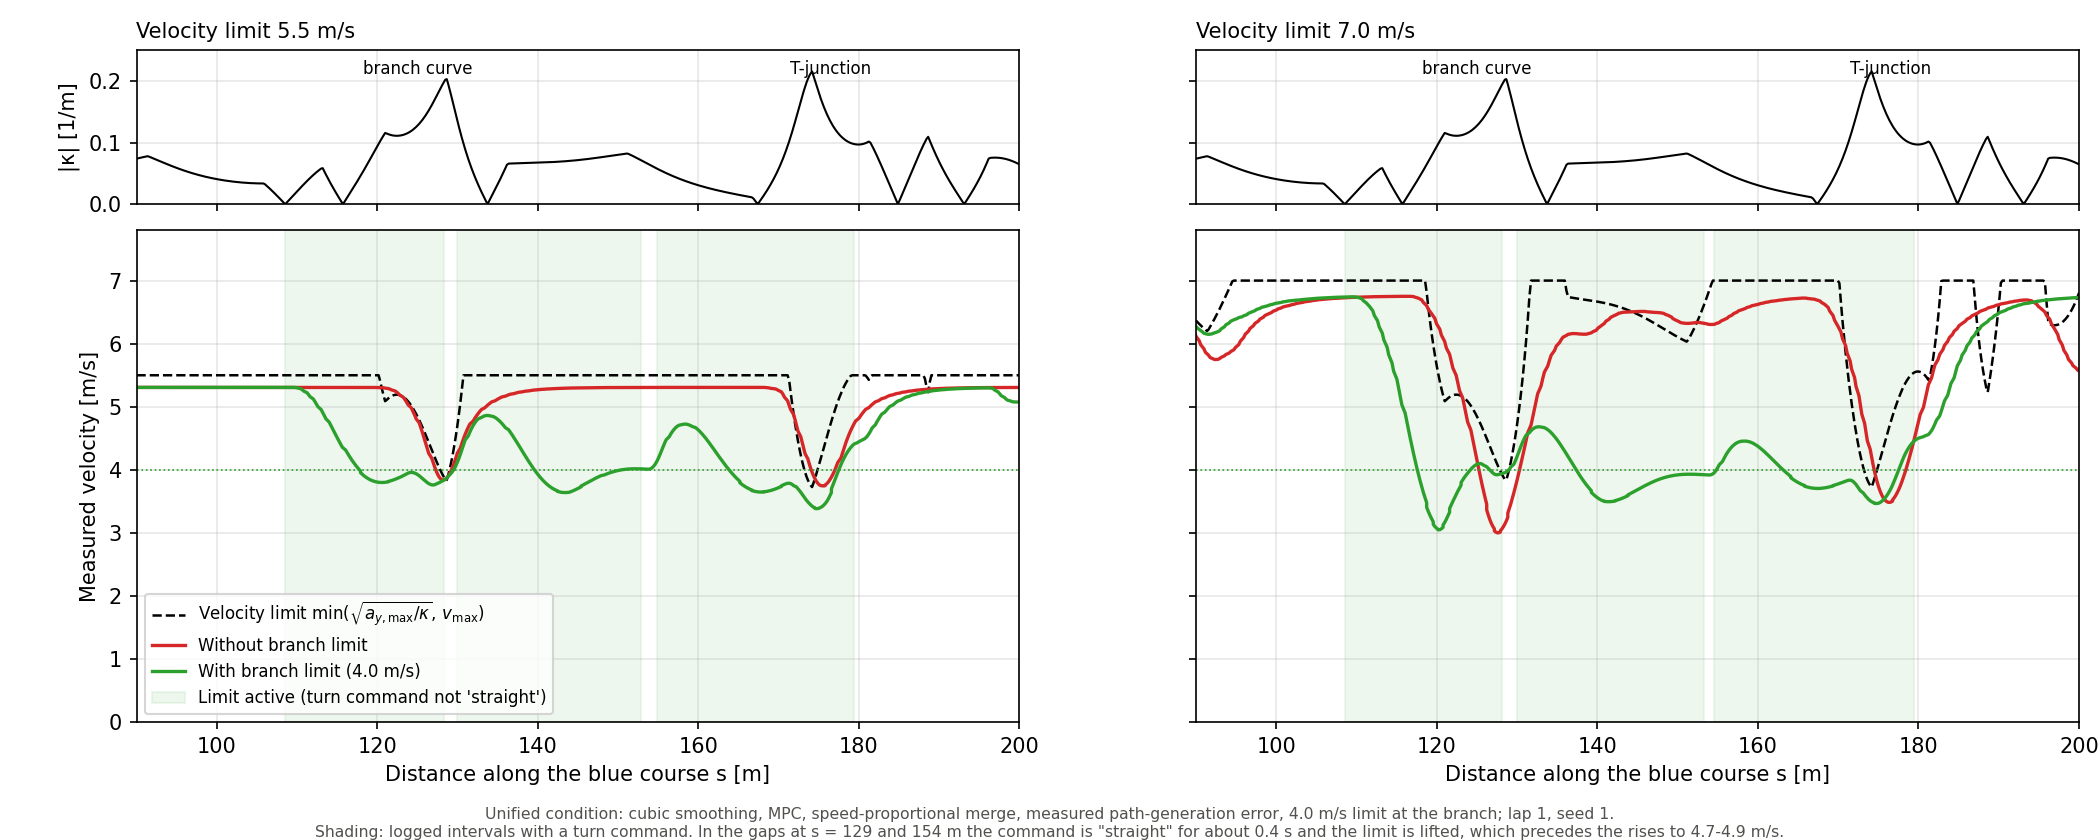
\includegraphics[width=0.95\textwidth]{images/sil_branch_speed_unified.png}
  \caption{Simulated vehicle speed around the branch curve and the T-junction of the blue course ($s=90$--$200$\,m) at upper speed limits of 5.5\,m/s (left) and 7.0\,m/s (right), without and with the branch speed reduction, in the unified conditions (cubic smoothing, measured error model, MPC, velocity-proportional merge length, branch speed reduction to 4.0\,m/s; lap 1, seed 1). Top: $|\kappa|$ of the course. Dashed line: speed limit $\min(\sqrt{a_{y,\max}/|\kappa|},\,v_{\max})$. Shaded: intervals in which the route instruction recorded by the simulation is not ``straight'', i.e., in which the speed limit is active. In this simulation the instruction briefly returns to ``straight'' at $s\approx 129$ and 154\,m (about 0.4\,s each), where the limit is released and the speed rises to 4.5--4.9\,m/s; whether the instruction of the real topological map has the same gaps is unconfirmed.}
  \label{fig:sil_branch}
\end{figure}

\subsection{経路生成の雑音}
\label{sec:noise_result}
理想的な経路生成（A8）は，雑音なし，認識距離20\,m，平滑化なしの3つを同時に変えた条件であるため，差を雑音だけの効果とは言えない．この条件でのラップタイムの短縮は0.5\,s以内（シード間の標準偏差の2倍以内）であった．青コースの最大横偏差は0.33〜0.39\,mと基準より大きいが，3つの変更のうち，雑音のない経路を平滑化を経由せず入力することによる経路のサンプリングの違いによると考えられ，雑音の有無の効果としては切り分けていない．経路点のサンプリングを弧長（0.2\,m等間隔）ではなく$x$基準にした参考条件（A8x：0.96\,m間隔の21行，A8y：0.2\,m間隔）では，ラップタイムが基準よりA8xで$+5.4$〜$+12$\,s，A8yで$+2.1$\,s以内遅くなり，A8xは赤の4.0\,m/sで0/5になる（本表には示さない）．本表のA8で弧長サンプリングを選んだのは，実装の平滑化出力の経路点が0.2\,m等間隔であることに合わせたためである．上限速度でラップタイムが決まる条件では，理想的な経路生成でもラップタイムはほとんど変わらなかった．

完走判定の閾値と雑音の大きさに対する結果の頑健性も確かめた．雑音の大きさを0.5倍，2倍にしても，基準は赤・青の全条件（4.0，5.5\,m/s）で5/5が完走し，ラップタイムは最大0.3\,s（青5.5\,m/sの2倍で52.7\,sから53.0\,s）しか変わらず，最大横偏差は雑音にほぼ比例した（0.5倍で0.08〜0.14\,m，2倍で0.23〜0.35\,m）．合流距離固定（A5）の赤コースは，雑音を半分にしても4.0\,m/sで2/5（最大横偏差1.49\,m），2倍では4.0，5.5\,m/sとも0/5であるが，5.5\,m/sで雑音を半分にすると5/5が完走し（1.07\,m，最悪1.46\,m），閾値の1.5\,mに近い．A4+A5の赤コースは全倍率で5/5（約1.1\,m，雑音の大きさに依存しない），青コースのA5とA4+A5は全倍率で0/5であった．完走判定の閾値を1.0，1.5，2.0\,mに変えると，基準は全閾値で5/5であり，青コースの基準（5/5）とA5（0/5）の対比は全閾値で保たれる．一方，赤コースのA5は，閾値2.0\,mでは4.0，5.5，7.0\,m/sで4/5，5/5，5/5，閾値1.0\,mでは全速度で0/5となり，完走率の対比が閾値に依存するため，その差は最大横偏差（基準0.2\,m以下，A5 1.4〜1.7\,m）で述べる．また，A4+A5は閾値に近く（最大横偏差は赤0.9〜1.1\,m，青1.7〜1.8\,m），閾値1.0\,mでは赤の4.0\,m/sが0/5（5.5\,m/sが3/5，7.0\,m/sが5/5），2.0\,mでは青が全速度で5/5になるため，A4+A5の完走の可否は，横偏差の0.5〜1.9倍のずれ（\ref{sec:sil_validity}節）で入れ替わりうる．

\subsection{停止減速度の分離}
\label{sec:stop_result}
赤コースの信号停止について，停止専用の減速度を分けた基準構成と，走行時の縦加速度3.0\,m/s$^2$と共通にした条件（A2）を比較した．信号停止の成否は，20\,Hzのログで$t>5$\,sかつ実速度が0.05\,m/s未満になった走行のうち，停止線からの行き過ぎ（停止位置から停止線を引いた値，停止線を越えた量を正．停止線はパイロンの3.3\,m手前，パイロンは$s=136$\,m）が1.0\,m以下のものを停止とし，$s=165$\,mまで一度も停止しなかった走行を通過とする．行き過ぎの許容量を入れない判定では，上限5.5\,m/s・検知距離9.3\,mの$+2.04$\,mの1本も停止に数えられるが，ここでは数えない．上限速度4.0\,m/sでの行き過ぎは，基準で$+0.78$\,m（$+0.46$〜$+0.86$\,m），A2で$+1.37$\,m（$+1.25$〜$+1.65$\,m）であり，分離によって行き過ぎは0.6\,m減る．SILの行き過ぎは真の停止線に対する値であるため，比べる実車の値は，4章の0.81\,m（認識が示す停止点に対する値）ではなく，真値基準の見積もり約1.2〜1.6\,m（$\pm 0.5$\,m，Fig.~\ref{fig:sil_stop}の説明を参照）である．分離なしのA2（$+1.37$\,m）はこの見積もりの範囲にあり，分離した基準（$+0.78$\,m）はそれより0.6\,m小さい（ただし10月12日の実車は計画の縦加速度が6.0\,m/s$^2$であり，A2の3.0\,m/s$^2$とは設定が異なる）．上限速度5.5\,m/sでは両条件とも0/5（4本は通過，1本は$+2.04$\,mで停止したが行き過ぎが1.0\,mを超える），7.0\,m/sでは5本すべてが通過した．この構成で信号停止を確認できたのは上限速度4\,m/sまでである．なお，本シミュレーションの信号停止はコーンの検知距離（最遠9.3\,m）の内側でのみ停止点を発行する実装であり，停止点はコーンの3.3\,m手前であるから，9.3\,mは停止点までの6.0\,mに相当する．この9.3\,mは追試で調整した値ではなく，10月12日の記録でコーンが最初に検出された距離（3回の接近で推定距離9.0〜9.5\,m）から定めたSILの検出モデルの既定値で，停止点までの距離6.0\,mは，実車で停止点が最初に発行された距離5.3\,m（10月12日）と6.98\,m（R2）の間にある．SILでは検知範囲内のコーンを毎フレーム位置誤差なしで検出し，揺らぎや欠落は入れていない．コーンの検知距離を15\,m（停止点まで11.7\,m）と20\,m（16.7\,m）に延ばした条件（Table~\ref{tab:signal_range}．実車の認識性能の予測ではなく改善案の感度分析として読む）では，5.5\,m/sと7.0\,m/sでも5本すべてが停止し，行き過ぎは15\,mで$-0.01$\,mと$+0.10$\,mであった．5.5\,m/sと7.0\,m/sのいずれも，検知距離9.3\,mで0/5，15\,mで5/5と全試行で結果が分かれたため，停止点までの距離の不足（遅れを含む停止距離に足りないこと）が5.5\,m/s以上で停止できない原因であると言える．

この機構を，停止点が初めて速度計画に現れた時点の必要減速度（検知時の実速度$v_0$と停止点までの距離$d_0$から$v_0^2/(2d_0)$）と，計画された減速度の記録から調べた（各3シード）．上限速度4.0\,m/sでは，必要減速度が0.45〜1.3\,m/s$^2$と小さく，検知直後は走行時の減速度1.5\,m/s$^2$が使われ，制動中は2.0〜2.3\,m/s$^2$まで上がり，減速曲線は残距離約5.3\,mから効き始めるため，検知距離（停止点まで5.7，11.5，16.4\,m）によらず同じ制動になり，行き過ぎ$+0.6$〜$+0.8$\,mは検知距離を延ばしても変わらない．この行き過ぎの内訳は，実速度が0.3\,m/s未満になる位置が停止線の$+0.2$\,m先で，続く速度指令0.13〜0.16\,m/sの這い寄りが約5\,s（4.7〜5.8\,s）続いて0.5〜0.6\,m進むことによる（縦PIDの停止直前の挙動が疑われるが，切り分けていない）．5.5，7.0\,m/sで検知距離が15\,m以上の場合は，必要減速度が0.87〜2.07\,m/s$^2$（20\,mを含む）で検知距離が制動距離を上回り，速度指令が停止線の0.9〜1.05\,m手前で0になって行き過ぎは約0\,mになる（ただし7.0\,m/s・20\,mは平均$+0.34$\,m（$-0.53$〜$+0.86$\,m）で，這い寄りが1.18\,m・7.5\,s生じた）．検知距離9.3\,mの5.5，7.0\,m/sでは，必要減速度が2.5〜4.4\,m/s$^2$と大きく，計画された減速度は検知直後の2.3，3.7\,m/s$^2$から制動中の最大3.9，4.0\,m/s$^2$と停止専用の上限4.0\,m/s$^2$近くまで上がるが，SILの車両モデルの減速の上限（3.5\,m/s$^2$）のもとでは実減速は最大3.3〜3.4\,m/s$^2$にとどまり，停止点までの距離が遅れを含む停止距離に足りず，停止できない．すなわち，停止できない原因は停止点までの距離が遅れを含む停止距離に足りないことである（\ref{sec:bottleneck}節の条件式でも，減速度3.6\,m/s$^2$と実効的な遅れでの切り替わりの速度は4.5〜5.6\,m/s）．計画の上限4.0\,m/s$^2$が車両の実減速（約3.4\,m/s$^2$）を上回ることが直接の原因とは断定しない．実車の同定値の減速の上限は3.6\,m/s$^2$，実測の最大は3.7〜4.4\,m/s$^2$であり（4章），実車では4.0\,m/s$^2$を実現できる可能性がある（\ref{sec:limitations}節）．

\begin{table}[H]
  \centering
  \caption{Overshoot of the stop position on the red course for different detection ranges of the cones that trigger the stop point (implemented SIL, 5 seeds; mean and range). The distance to the stop point is the detection range minus 3.3\,m, because the stop point is placed 3.3\,m before the cone. The overshoot is positive beyond the stop line. A run is counted as stopped when the speed fell below 0.05\,m/s with an overshoot of at most 1.0\,m, and as passed when it never stopped before $s=165$\,m.}
  \label{tab:signal_range}
  \small
  \begin{tabular}{L{3.2cm}L{3.0cm}L{3.6cm}L{3.6cm}}
    \toprule
    検知距離（停止点まで） & 4.0\,m/s & 5.5\,m/s & 7.0\,m/s \\
    \midrule
    9.3\,m（6.0\,m，現行） & $+0.78$\,m（平均，範囲$+0.46$〜$+0.86$，5/5停止） & 0/5停止（4本は通過，1本は$+2.04$\,mで停止） & 0/5停止（5本は通過） \\
    15\,m（11.7\,m） & $+0.78$\,m（平均，範囲$+0.66$〜$+0.86$，5/5） & $-0.01$\,m（5/5） & $+0.10$\,m（5/5） \\
    20\,m（16.7\,m） & $+0.70$\,m（平均，範囲$+0.46$〜$+0.86$，5/5） & $-0.09$\,m（5/5） & $+0.34$\,m（5/5，$-0.53$〜$+0.86$） \\
    \bottomrule
  \end{tabular}
\end{table}

Fig.~\ref{fig:sil_stop}に，10月12日の停止の記録に合わせた車両モデルによる1次元の閉ループ計算で，速度計画の設定を変えたときの行き過ぎを示す．この図の行き過ぎは真の停止位置に対する値であり，4章の0.81\,m（認識が示す停止点に対する値）とは基準が異なる．認識が示す停止点は，近距離（3\,m付近）で単眼の深度が約11\%過大に見積もられるため，真の停止線より約0.3〜0.4\,m先に出る．また，真の停止線の位置自体をコーンの検出位置から代理的に求めており，$\pm 0.5$\,mの不確かさがある．単眼の深度は，近距離では約11\%過大に見積もられる一方，遠距離では圧縮され（真の11.5\,mが約5.4\,m），距離に対して非線形である．これらから，真の停止位置に対する実車の行き過ぎは，認識基準の0.81\,mに深度の過大による0.3〜0.4\,mを加えた約1.2\,mから，代理の停止線に対する値1.64\,m（$\pm 0.5$\,m）までの約1.2〜1.6\,mと見積もられ，図の現行設定（10月12日の設定，S3で$+1.8$\,m）は，この範囲の上端（$\pm 0.5$\,mを含む）に入る．S3は10月12日の停止3に相当する条件で，停止点が最初に発行されたときの真の停止点までの距離（D0）を11.5\,mとし，単眼深度の圧縮により認識が示す距離は約5.4\,m（4章の実測は約5.3\,m）になる．減速側の計画値を3.0\,m/s$^2$に下げるだけ（B）では，完全な認識（深度の圧縮なし）の場合に行き過ぎが4，5，6\,m/sで約1.5〜1.6\,m残る（S3では約0.3\,m）．停止距離への遅れの補償（$0.4v$）と深度の補正を組み合わせる（R+G）と，完全な認識の4，5，6\,m/sで$-0.16$，$-0.31$，$-0.65$\,mとなり，6\,m/sの$-0.65$\,mを除いて$\pm 0.5$\,mの範囲に入る．停止点を絶対位置で保持すると手前側（負，$-0.74$〜$-1.08$\,m）になる．4章で示した実車の行き過ぎの主因は車両の遅れであり，減速専用の減速度は制動を早く始めることで遅れを一部補償するが，停止点までの距離の不足と遅れを完全には補えない．

\begin{figure}[H]
  \centering
  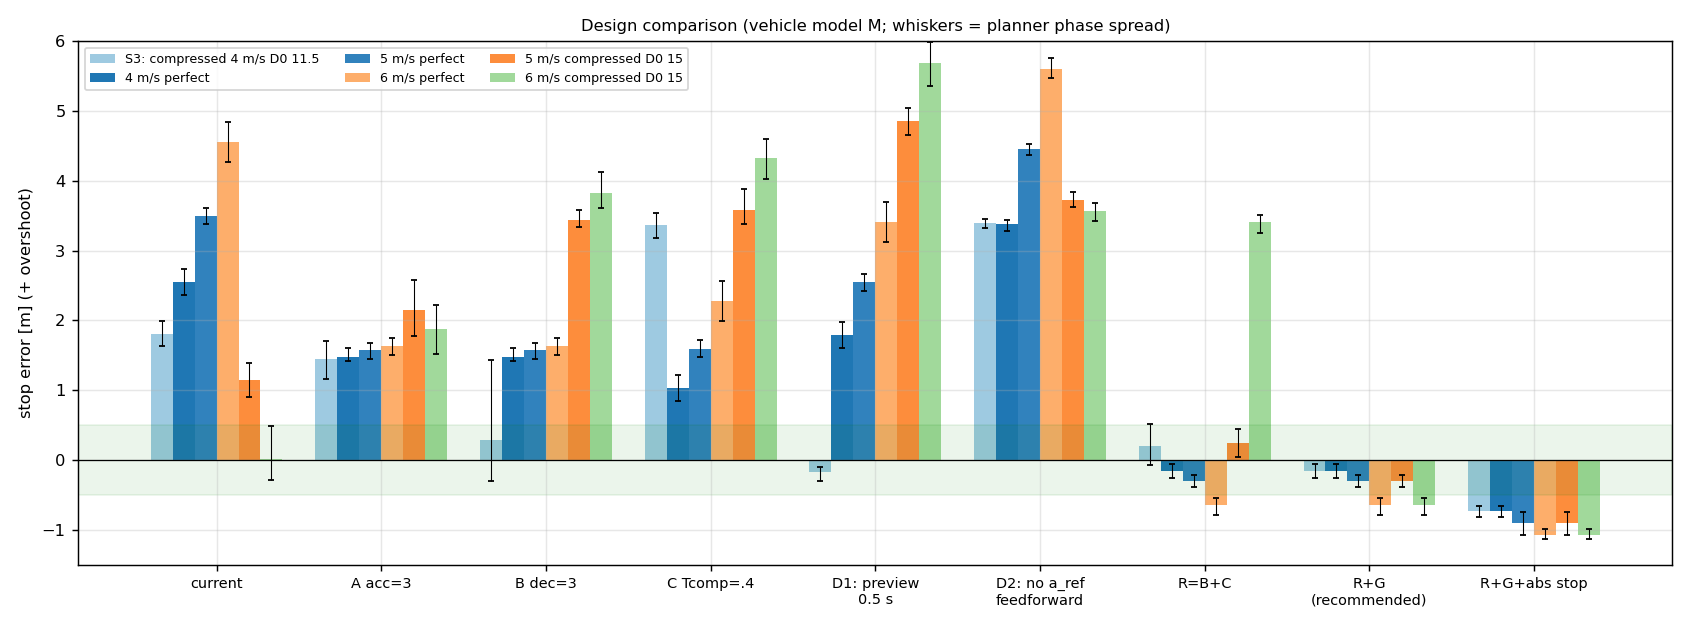
\includegraphics[width=0.95\textwidth]{images/sil_stop_design.png}
  \caption{Overshoot of the true stop position for different velocity-planning settings (one-dimensional closed-loop calculation; M is the vehicle model fitted to the stop on October 12 (dead time 0.27\,s, first-order lag 0.39\,s); bars are the mean over four planner phases and whiskers the range). Settings: current (the setting of October 12: planned acceleration 6.0\,m/s$^2$, preview 0.3\,s); A: planned acceleration and deceleration 3.0\,m/s$^2$; B: planned deceleration 3.0\,m/s$^2$ only; C: delay compensation of the stop distance by $0.4v$; D1: preview 0.5\,s; D2: no acceleration feed-forward; R: B and C; R+G (recommended): R with inverse correction of the compressed monocular depth; R+G+abs stop: R+G with the stop point held at an absolute position. D0 is the distance from the vehicle to the stop point when the stop point is first issued. Legend: S3, the condition equivalent to stop 3 of October 12 (perception compressed as in that stop, D0 = 11.5\,m, 4\,m/s); perfect perception at 4, 5, and 6\,m/s; and compressed perception with D0 = 15\,m at 5 and 6\,m/s.}
  \label{fig:sil_stop}
\end{figure}

\subsection{自己位置の姿勢の欠落に対する頑健性}
\label{sec:yawfreeze_result}
4章で実車の失敗の主因であった慣性航法装置の出力の途絶を，シミュレーションに注入して要素の頑健性を評価した．各ノードに与える自己位置の姿勢を，青コースの急カーブの約2\,s手前（$s\approx 108$\,m）から2，5，10\,s凍結し（位置は凍結した姿勢で積分し，角速度は途絶させる），復帰時に姿勢だけを真値に戻す．基準構成（MPC）とPure Pursuit法について，上限速度5.0\,m/s，各5シードの結果をTable~\ref{tab:yawfreeze}に示す．凍結10\,sまでは両方の追従制御で完走を失わず，凍結なしに対する最大横偏差（平均）の増加は，MPCで$-0.01$（2\,s），$+0.31$（5\,s），$+0.22$\,m（10\,s），Pure Pursuit法で$0$，$+0.16$，$+0.33$\,mと約0.3\,mにとどまり，最悪値の増加は最大で約0.5\,mであった．舵角の指令値の変化率は凍結中と復帰直後に，凍結なしの参照値の1.5〜4.7倍に増え，5\,sと10\,sの凍結では復帰時の姿勢の跳びがシードごとに32〜67$^\circ$であり，舵角の指令値に最大400\,$^\circ$/sを超える急変が生じたのは5\,s凍結（MPC 445，Pure Pursuit法 411\,$^\circ$/s）のみで，10\,s凍結では206，297\,$^\circ$/sであった．これは，復帰直後に舵角の振動が大きいという4章の観測と，舵角の急変の点で整合する．ただし，実車で蛇行に至ったR4，R5，R7（赤コース）は再現しておらず（注入は青コースで，凍結中も復帰後も完走），注入した凍結が実車の欠落を代表するかは確認できていない．MPCの5\,s凍結（$0.51\pm 0.12$\,m）と10\,s凍結（$0.42\pm 0.08$\,m）の差はWelchの検定で$p=0.20$であり有意でない．5\,sの復帰（$s\approx 129$\,m）がカーブの頂点に当たり，10\,sの復帰（$s\approx 150$\,m）が直線寄りであることが差の向きに働いたと考えられるが，断定はしない．Pure Pursuit法は凍結がなくても横偏差が0.79\,mと大きく，10\,sの凍結で最悪1.33\,mと完走の判定に近づく．なお，この注入は自己位置の姿勢のみを対象とし，実車で同時に生じた装置の再起動によるバイアスや方位の変化は含まない．

\begin{table}[H]
  \centering
  \caption{Robustness to a frozen heading of the localization (implemented SIL, blue course, 5\,m/s limit, 5 seeds): completion, mean (worst) maximum lateral deviation, and mean steering-command rate during the freeze and in the 3\,s after recovery.}
  \label{tab:yawfreeze}
  \small
  \begin{tabular}{llrrrr}
    \toprule
    追従制御 & 凍結 & 完走 & 最大横偏差 [m] & 凍結中の舵角変化率 [$^\circ$/s] & 復帰後3\,s [$^\circ$/s] \\
    \midrule
    MPC & なし & 5/5 & 0.20 (0.27) & 6.5〜7.1 & 6.3〜7.5 \\
    MPC & 2\,s & 5/5 & 0.19 (0.21) & 9.8 & 16.3 \\
    MPC & 5\,s & 5/5 & 0.51 (0.70) & 19.8 & 28.4 \\
    MPC & 10\,s & 5/5 & 0.42 (0.51) & 15.5 & 18.1 \\
    Pure Pursuit法 & なし & 5/5 & 0.79 (0.81) & 3.4〜4.4 & 3.4〜6.5 \\
    Pure Pursuit法 & 2\,s & 5/5 & 0.79 (0.81) & 6.3 & 9.1 \\
    Pure Pursuit法 & 5\,s & 5/5 & 0.95 (1.11) & 15.2 & 21.1 \\
    Pure Pursuit法 & 10\,s & 5/5 & 1.12 (1.33) & 18.1 & 16.1 \\
    \bottomrule
  \end{tabular}
\end{table}

\subsection{経路生成の認識距離と曲率}
\label{sec:horizon_result}
経路生成が高速域で制約要因になりうる機構には，認識距離の不足と，平滑化による曲率の過小評価の2つがある．認識距離は，4章で示したように中央値8.1\,mで25\%のフレームで6\,m未満であり，カーブでは6\,m程度，直線では9\,m程度である．Fig.~\ref{fig:sil_horizon}に，10月12日の記録に対する，経路生成の出力と平滑化後の経路の曲率を，実際に走行した曲率に対する比として前方距離ごとに示す．10月12日時点の2次多項式で12\,mまで当てはめた平滑化では，曲率比は2.5\,m先で0.49，4\,m先で0.47，6\,m先で0.41である．3次多項式では2.5\,m先で0.79，4\,m先で0.53と近傍では改善するが，6\,m先では0.19と悪化する．同図の右に示すように，曲率比が0.47のとき，横加速度の設定値3.0\,m/s$^2$で計画した速度での実際の横加速度は6.4\,m/s$^2$となり，摩擦限界（約6\,m/s$^2$）を超える．

\begin{figure}[H]
  \centering
  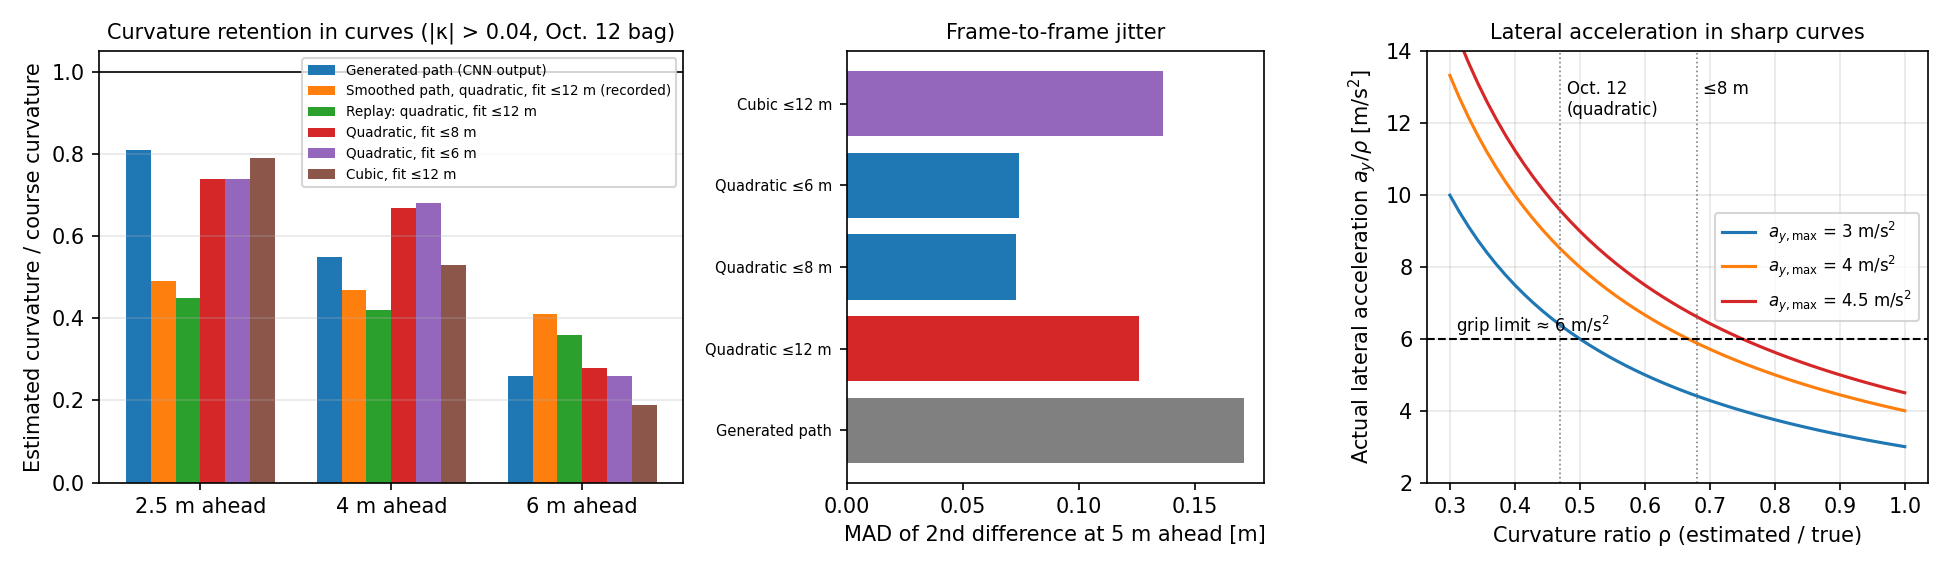
\includegraphics[width=0.95\textwidth]{images/sil_curvature_horizon.png}
  \caption{Curvature of the generated and smoothed paths relative to the driven curvature at 2.5, 4, and 6\,m ahead (left, October 12 record), frame-to-frame jitter at 5\,m ahead (center), and the actual lateral acceleration in a sharp curve versus the curvature ratio for planned lateral-acceleration limits of 3, 4, and 4.5\,m/s$^2$ (right; the vertical line labeled ``Oct. 12 (quadratic)'' marks the curvature ratio of the quadratic smoothing on October 12).}
  \label{fig:sil_horizon}
\end{figure}

\ref{sec:bottleneck}節の条件式によれば，7\,m/sで交差点の急カーブに進入するために必要な先読み距離は8.5\,m（減速度3.0\,m/s$^2$，遅れ0.38\,s）であり，認識距離9\,mでは満たされるが6\,mでは満たされない．そこで，前方6\,m以内にカーブ（$|\kappa|>0.04$\,1/m）がある場合に認識距離を6\,mに短縮する条件（6/9\,m切替．走行距離のうち赤で42\%，青で63\%の区間で認識距離が6\,mになり，実車の「25\%のフレームで6\,m未満」より厳しい）で，基準構成と分岐での速度抑制なし（A7）を上限速度5.0〜7.0\,m/sで走行させた（Fig.~\ref{fig:sil_horizon6}，各5シード）．その結果，赤・青，A7の有無，認識距離9\,m一定と6/9\,m切替のすべての条件で5本すべてが完走し，最大横偏差は0.14〜0.28\,m，ラップタイムの差は0.5\,s以内，最大横加速度（平均）の変化は$-0.2$〜$+0.4$\,m/s$^2$にとどまった（最大横加速度の変化は5.0〜7.0\,m/sの範囲の値であり，8\,m/s以上では最大横加速度が摩擦限界の6\,m/s$^2$に達する条件がある）．さらに，認識距離を4.5\,mに縮めた条件（実測誤差モデルの行，6.0〜8.0\,m/s，赤・青の基準と青のA7）や，上限速度8.0\,m/sの6/9\,m切替でも5本すべてが完走した．実測誤差モデルの行（21行，前方0.77〜8.89\,m）では，6/9\,m切替で欠けるのは最遠の8.89\,mの1点だけで，5.83\,mまでの20点は残る（4.5/9\,m切替では5.83\,mと8.89\,mの2点が欠ける）．そこで，行構成を0.5\,m間隔（0.8〜8.8\,m，17行）に密にし，6\,m以遠の点をすべて消す条件（密な行・6/9\,m切替）でも確認したところ，基準構成では6.0〜9.0\,m/sのすべてで5本が完走し，最大横偏差は認識距離9\,m一定の0.44\,mに対して6/9\,m切替で0.36〜0.45\,m，最大横加速度の差は0.5\,m/s$^2$以内であった．9.0\,m/sで完走が崩れたのは，実測誤差モデルの行ではA7・9\,m一定（3/5，最大横偏差1.32\,m），密な行ではA7・6/9\,m切替（2/5，1.52\,m）の2条件だけである．実測誤差モデルの行では6/9\,m切替は9.0\,m/sでも基準，A7とも5/5であり，密な行でもA7・9\,m一定は5/5である．すなわち，認識距離の短縮が完走を悪くする向きと良くする向きの両方が現れ，その差は5シードのばらつきの範囲にある．

悲観モデル（\ref{sec:sil}節）と3次の組合せでも，抑制ありの基準構成は赤・青とも8.0\,m/sまで5/5が完走し，完走が崩れるのはA7の8.0\,m/sのみであった（9\,m一定で2/5，6/9\,m切替で1/5．この2条件の差は5本では区別できない）．悲観モデルは最大横偏差を増やす（赤の8.0\,m/sで，実測誤差モデルの0.23\,mに対し9\,m一定で1.2\,m，6/9\,m切替で1.0\,m）が，6/9\,m切替の寄与（9\,m一定との差0.4\,m以内）はそれより小さい．

認識距離6\,mでも完走が保たれる理由として，3次多項式の平滑化が認識距離の外へ曲率を外挿し，その先のカーブを速度計画に与えるためという説明が考えられた．そこで，認識距離9\,m一定の条件で，平滑化の出力を9\,mで打ち切り，9\,m以遠の外挿部を速度計画と局所経路計画に渡さない条件を試した（青は基準とA7の7.0，8.0，9.0\,m/s，赤は基準の7.0，8.0\,m/sのみ，各5シード．6/9\,m切替との組合せは未実施）．完走，ラップタイム（差は0.2\,s以内．A7の9.0\,m/sのみ$-0.8$\,s），交差点カーブの最大横加速度（差は0.4\,m/s$^2$以内）はいずれも打ち切りで変わらず，9\,m以遠の外挿は結果に影響しなかった．さらに6\,mまで打ち切ると（青，基準とA7，7.0，8.0\,m/s，9\,m一定と6/9\,m切替，各5シード），完走（全16セルで5/5）とラップタイム（差は0.6\,s以内）は変わらないが，最大横偏差は基準で0.20\,mから0.48\,m（7.0\,m/s），0.24\,mから0.58\,m（8.0\,m/s），A7で0.28\,mから0.72\,m，0.28\,mから0.97\,mに増え，A7の交差点カーブの最大横加速度は7.0\,m/sで$4.0\pm 0.4$から$5.2\pm 0.5$\,m/s$^2$（9\,m一定），$5.0\pm 0.5$から$5.3\pm 0.4$\,m/s$^2$（6/9\,m切替）に上がる（8.0\,m/sは打ち切りなしでも5.5〜6.0\,m/s$^2$で摩擦限界に近い）．基準（抑制あり）の交差点カーブは2.4〜2.6\,m/s$^2$のままである．ただし，6\,m打切りでは局所経路計画の合流終点が参照経路の終端にクランプされ（終端の位置は自車位置の20\,m先と参照経路の長さの小さい方，合流先の位置は終端と自車位置から合流距離先の小さい方），局所経路が5〜6\,m（合流距離より短いフレームが83\%）になるため，この介入は外挿の除去と局所経路の短縮の複合効果である．したがって，3次の外挿が先読みを補う効果は，9\,m打切りでは現れず，6\,mまで短くすると最大横偏差と交差点カーブの横加速度に現れるが，完走とラップタイムを変える大きさではない．認識距離6\,mでも完走が保たれたのは，速度計画の横加速度の設計上限（3.0\,m/s$^2$）と摩擦限界（6.0\,m/s$^2$）の間の余裕と，完走判定の閾値（1.5\,m）の余裕によると考えられる．

条件式が予測するのは，速度計画が横加速度の設計上限3.0\,m/s$^2$を守れなくなる速度であるから，シミュレーションと比べる指標は完走ではなく横加速度である．A7の交差点カーブの最大横加速度（平均）は，上限速度5.5\,m/sで3.0\,m/s$^2$を超え始め（9\,m一定で3.4，6/9\,m切替で3.3，\ref{sec:branch_result}項のTable~\ref{tab:branch_ay}），この速度は条件式の6\,mの見積もり（5.2〜6.0\,m/s）の範囲内にある．ただし，条件式が予測する認識距離への依存（6\,mから9\,mで約1\,m/s）は，超過の開始速度には現れず，7\,m/s以上の超過量（9\,m一定で4.0，6/9\,m切替で5.0\,m/s$^2$，8.0\,m/sで5.5と6.0）にのみ現れた．分岐カーブ（半径約4.9\,m）では，A7の最大横加速度が5.0\,m/sで既に$3.2\pm 0.1$\,m/s$^2$となる（条件式の見積もり5.3〜6.1\,m/s）．実測誤差モデルの5\,m以遠は5.83\,mと8.89\,mの2行だけで，8.89\,mの雑音が大きいため，実効的な認識距離が約6\,mとなっている可能性がある．摩擦限界6.0\,m/s$^2$に達するシードが現れるのは7.5\,m/s以上であるが，完走は実測誤差モデルでは8.5\,m/sまで5/5（9.0\,m/sで3/5）で保たれ，摩擦限界に達する7.5\,m/s以上でも完走が保たれたのは，完走判定の閾値（1.5\,m）の余裕による．

\begin{figure}[H]
  \centering
  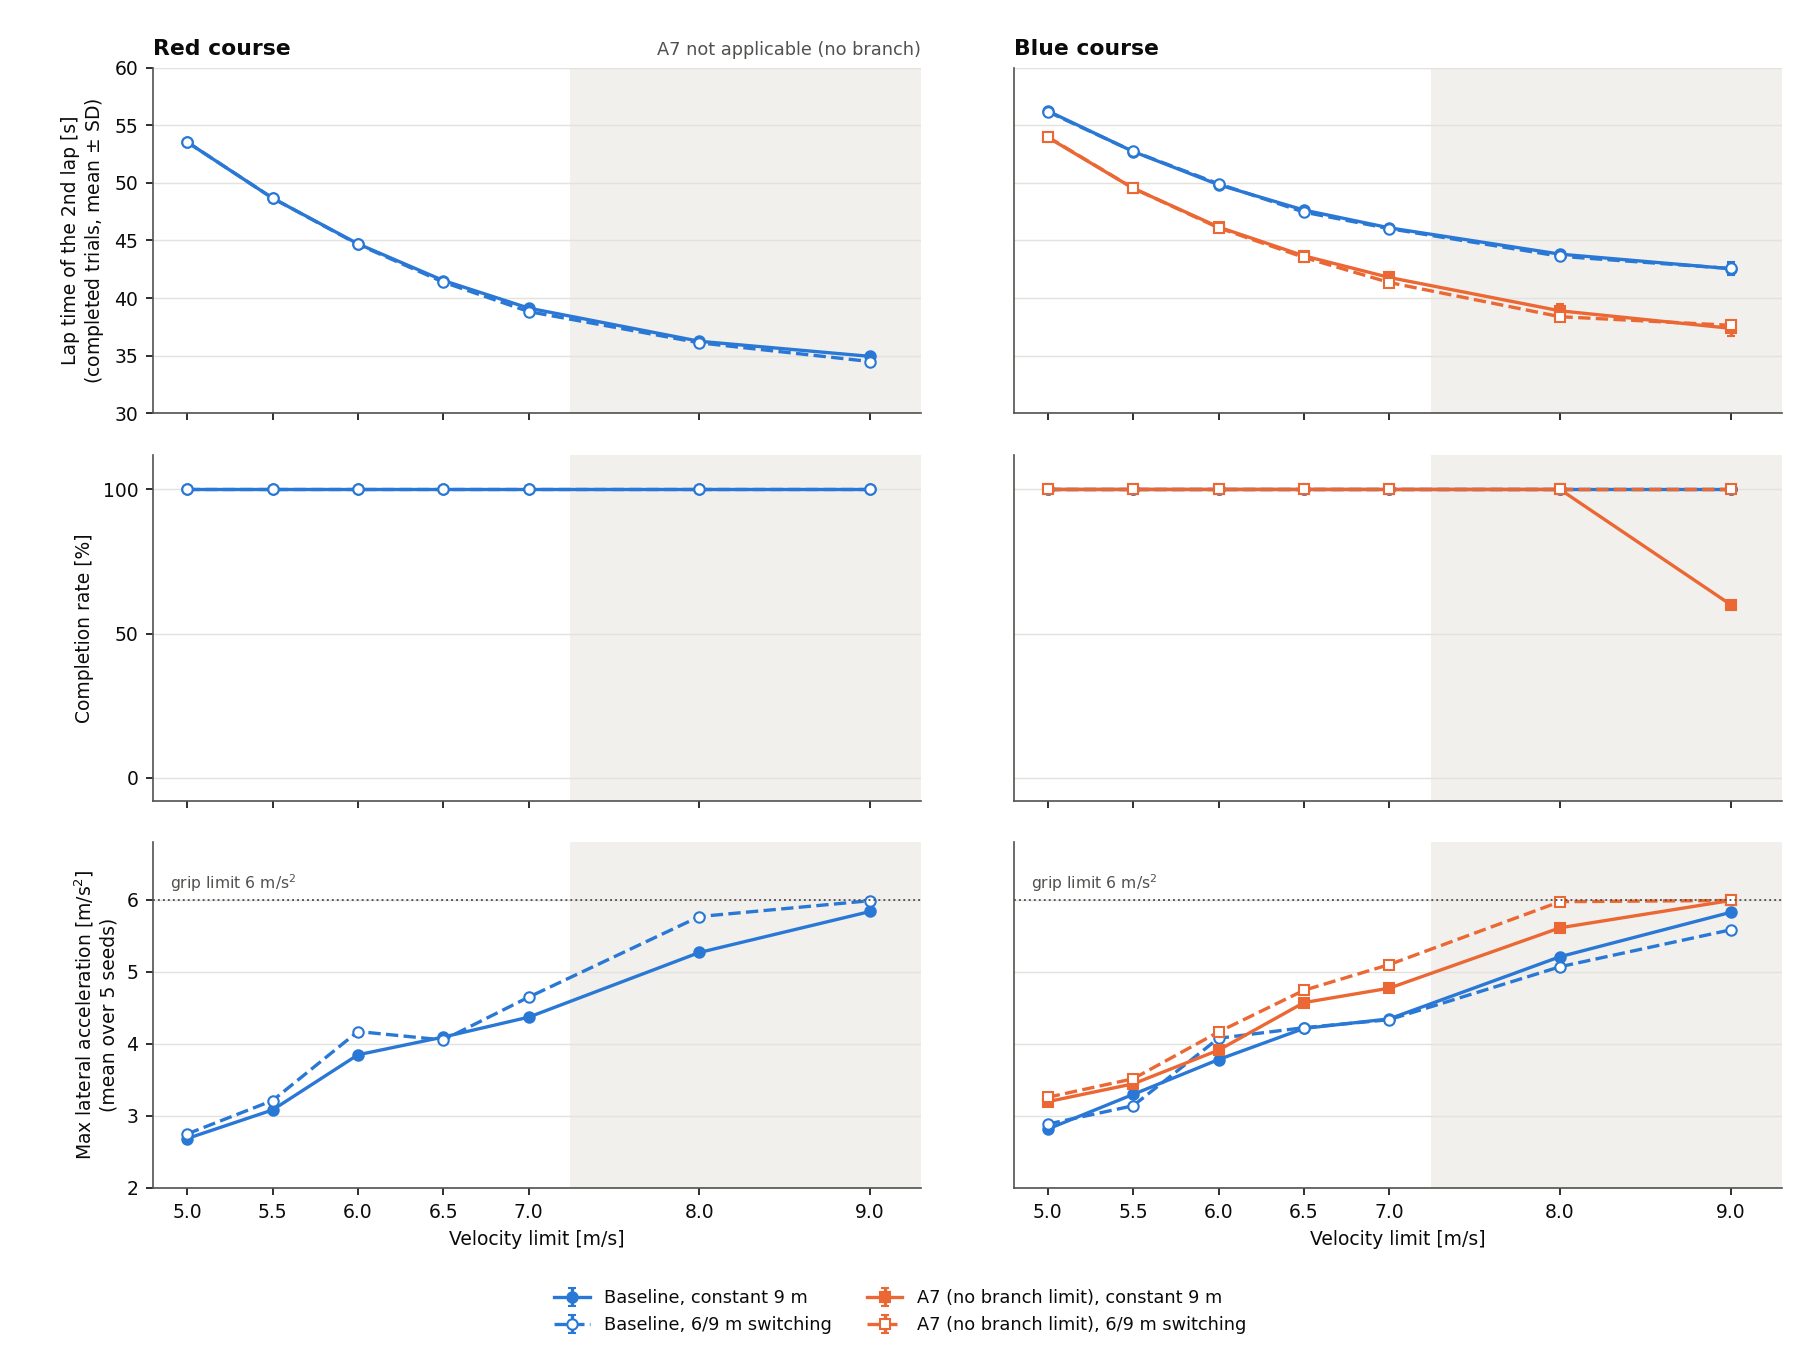
\includegraphics[width=0.95\textwidth]{images/sil_horizon6.png}
  \caption{Effect of shortening the recognition distance to 6\,m in curves (implemented SIL, 5 seeds): second-lap time (top), completion rate (middle), and maximum lateral acceleration over the whole lap (bottom, mean over 5 seeds) versus the upper speed limit, for a constant 9\,m and for the 6/9\,m switching, with and without the branch speed reduction (A7 is not applicable to the red course because it has no branch). The maximum lateral acceleration in the bottom panel is the maximum over the whole lap, not only in the intersection curve. The shaded range (8.0 and 9.0\,m/s) lies beyond the upper speed limits of the unified conditions.}
  \label{fig:sil_horizon6}
\end{figure}

\section{上限速度の段階と制約要因}
\label{sec:bottleneck}
4章の実車走行と本章のシミュレーションから，上限速度の段階ごとにラップタイムと完走を制約する要因をTable~\ref{tab:bottleneck}にまとめる．表には根拠の種類（実車の観測か，シミュレーションの予測か）を併記する．4\,m/sでは3周の走行が行え，ラップタイムの内訳は4章の\ref{sec:decomp_result}節に示した．5\,m/sでは，実車では自己位置推定の入力欠落と経路選択の初期化の不備が先に現れ，要素の設計の関与が特定できたのは2本（B7，R3）にとどまった（主因不明のB3，B4，B9は分岐の指示後の逸脱であり，設計の関与を排除できない）．シミュレーションでは，基準構成が赤・青とも7.0\,m/sまで完走する一方，赤コースの信号停止は，コーンの検知距離9.3\,m（停止点まで約6\,m）では5.5\,m/s以上で成立せず（行き過ぎ1.0\,m以下を停止として0/5），15\,mでは5.5，7.0\,m/sとも5/5であった．実車は従動輪のシミーにより6\,m/sを超えて走行できないため，6\,m/s以上の行は，車両モデルの同定範囲外（シミーを含まない）の予測である．

\begin{table}[!t]
  \centering
  \caption{Limiting factors of the lap time and completion by upper speed limit, with the type of evidence.}
  \label{tab:bottleneck}
  \small
  \setlength{\tabcolsep}{4pt}
  \begin{tabular}{lL{3.4cm}L{7.6cm}L{2.2cm}}
    \toprule
    上限速度 & 実車の観測 & シミュレーションの予測 & 根拠 \\
    \midrule
    4\,m/s & R2，R8は3周完走，B1は2.97周．内訳はTable~\ref{tab:decomp} & 完走．信号停止の行き過ぎ$+0.8$\,m & 実車・SIL \\
    5\,m/s & 自己位置推定の入力欠落，経路選択の初期化の不備（8本）．要素の設計の関与が特定できたのはB7の1本（主因不明のB3，B4，B9は設計の関与を排除できない） & 完走（赤・青）．合流距離を固定すると青で失敗（0/5，赤は3/5．A5は4.0，5.5，7.0\,m/sのみ実施し，5.5\,m/sの値） & 実車・SIL \\
    5.5\,m/s & 車体のヨー外乱と再計画・回避判断の相互作用（1本） & 完走（赤・青）．赤の信号停止は，コーンの検知距離9.3\,m（停止点まで約6\,m）では0/5，15\,m（約12\,m）では5/5 & 実車・SIL \\
    6\,m/s以上 & 従動輪のシミーにより走行不可 & A7（青，分岐での速度抑制なし）は7.0\,m/sまで完走する．A7の交差点カーブの横加速度は5.5\,m/s以上で設計上限3.0\,m/s$^2$を超え，この速度は条件式の6\,mの見積もり（5.2〜6.0\,m/s）の範囲内にあるが，認識距離への依存は開始速度には現れなかった．摩擦限界6.0\,m/s$^2$に達するのは7.5\,m/s以上で，完走は実測誤差モデルでは8.5\,m/sまで5/5，9.0\,m/sで3/5（完走判定の閾値の余裕による）．赤の信号停止は7.0\,m/sで，検知距離9.3\,mでは0/5，15\,mでは5/5 & SILのみ（同定範囲外，シミーなし） \\
    \bottomrule
  \end{tabular}
\end{table}

制約が切り替わる速度は，速度に依存する要求とシステムの固定された能力の比較として見積もることができる．Table~\ref{tab:thresholds}に，各制約を不等式で表し，同定値を与えて求めた切り替わりの速度$v^*$を示す．停止については，停止点までの距離$d_{\mathrm{stop}}$（R2の6.98\,mとSILの約6\,m）に対し，必要な停止距離は$v\tau + v^2/(2b)$で表され，これが$d_{\mathrm{stop}}$に等しくなる速度$v^*=-b\tau+\sqrt{b^2\tau^2+2bd_{\mathrm{stop}}}$が切り替わりの速度である．ここで$\tau$は系の実効的な遅れ，$b$は減速度である．遅れの代表値は，認識から制御までの遅延0.106\,sと車両のむだ時間0.20〜0.27\,sの和0.31〜0.38\,sのうち上端の0.38\,sとする．並進速度の一次遅れ$T=0.39$〜$0.65$\,sは減速の開始をほぼ$T$だけ遅らせ，速度計画の0.3\,s先の参照はそれを0.3\,s早めるため，実効的な遅れは$\tau_{\mathrm{eff}}\approx 0.38+T-0.3=0.47$〜$0.73$\,sと見積もられる．以下の$v^*$は$d_{\mathrm{stop}}=6$〜7\,mの範囲で示す．速度計画の停止減速度1.5\,m/s$^2$では$v^*\approx 3.7$〜$4.0$\,m/s（$\tau=0.38$\,s），$3.3$〜$3.9$\,m/s（$\tau_{\mathrm{eff}}$），車両の減速の上限3.6\,m/s$^2$では$v^*\approx 5.4$〜$5.9$\,m/s（$\tau=0.38$\,s），$4.5$〜$5.6$\,m/s（$\tau_{\mathrm{eff}}$）となる．4\,m/sで行き過ぎが残り，5.5\,m/s以上で検知距離9.3\,mでは停止できないというシミュレーションの結果は，行き過ぎの有無の点では$\tau_{\mathrm{eff}}$を用いた見積もりと矛盾しないが，機構は異なる．4\,m/sの行き過ぎは停止直前の速度指令の這い寄りが主因で検知距離に依存せず（\ref{sec:stop_result}項），条件式の遅れを含む停止距離とは別の要因である．5.5\,m/s以上で検知距離9.3\,mでは，停止点までの距離が遅れを含む停止距離に足りず，減速度3.6\,m/s$^2$の見積もり（4.5〜5.6\,m/s）と整合する．カーブの先読みについては，認識距離$d_{\mathrm{vis}}$に対し，カーブの速度$v_c=\sqrt{a_{y,\max}/\kappa}$まで減速するのに必要な距離$v\tau + (v^2-v_c^2)/(2b)$を比べる．交差点の半径4.6\,m，$a_{y,\max}=3.0$\,m/s$^2$（$v_c=3.7$\,m/s），$b=3.0$\,m/s$^2$では，$d_{\mathrm{vis}}=6$\,mで$v^*\approx 6.0$\,m/s（$\tau=0.38$\,s）または$5.2$〜$5.8$\,m/s（$\tau_{\mathrm{eff}}$），9\,mで$7.2$\,m/sまたは$6.3$〜$6.9$\,m/sである．条件式が予測するのは，速度計画が$a_{y,\max}=3.0$\,m/s$^2$を守れなくなる速度であり，比べる指標は完走ではなく横加速度である．A7の交差点カーブの最大横加速度（平均）は，上限速度5.0\,m/sで2.9，5.5\,m/sで3.4（最大3.8），6.0\,m/sで3.8，7.0\,m/sで4.0\,m/s$^2$であり，3.0\,m/s$^2$を超え始める5.5\,m/sは，認識距離6\,mの見積もり（5.2〜6.0\,m/s）の範囲内にある（Table~\ref{tab:branch_ay}）．ただし，条件式が予測する認識距離への依存（6\,mから9\,mで約1\,m/s）は，超過の開始速度には現れず（認識距離9\,m一定でも6/9\,m切替でも5.5\,m/s），7\,m/s以上の超過量（9\,m一定で4.0，6/9\,m切替で5.0\,m/s$^2$．8.0\,m/sで5.5と6.0）にのみ現れた．分岐カーブ（半径約4.9\,m）では，A7の最大横加速度が5.0\,m/sで既に$3.2\pm 0.1$\,m/s$^2$となる（見積もり5.3〜6.1\,m/s）．実測誤差モデルの5\,m以遠は5.83\,mと8.89\,mの2行だけで，8.89\,mの雑音が大きいため，実効的な認識距離が約6\,mとなっている可能性がある．摩擦限界6.0\,m/s$^2$に達するシードが現れるのは7.5\,m/s以上，完走が崩れるのは9.0\,m/s（3/5）であり，完走は実測誤差モデルでは8.5\,m/sまで5/5で保たれたが，摩擦限界に達する7.5\,m/s以上でも完走が保たれたのは完走判定の閾値（1.5\,m）の余裕による．抑制ありの基準構成は，全速度で交差点カーブの横加速度が2.5〜2.9\,m/s$^2$にとどまり，先読みの制約は試されていない．また，試した上限速度の刻み（0.5〜1.5\,m/s）は$\tau$の取り方による$v^*$の幅と同程度であり，この一致は条件式の独立な検証とは言えない．グリップについては，速度計画が$a_{y,\max}=3.0$\,m/s$^2$で計画する限り$v^2\kappa$は摩擦限界$\mu g\approx 6$\,m/s$^2$に達せず，曲率比$\rho$が$a_{y,\max}/(\mu g)=0.5$を下回る場合にのみ超える．Fig.~\ref{fig:sil_horizon}の2次の平滑化の曲率比0.41〜0.49はこの閾値の近傍にある．一方，3次の6\,m先の曲率比は0.19と閾値を大きく下回るが，摩擦限界の超過には直結しない．これは，速度計画が使う曲率が平滑化後の経路から毎周期更新され，カーブへの進入後は近傍（6\,m未満）の曲率で減速が決まるためと推定される（確認はしていない）．舵角については，半径4.6\,mに必要な舵角$\arctan(L\kappa)\approx 8.7^\circ$（$L=0.70$\,m）は制限の$15^\circ$より小さく，定常では制約にならない．

\begin{table}[!t]
  \centering
  \caption{Speed-dependent requirements, fixed capabilities, and the estimated switching speeds.}
  \label{tab:thresholds}
  \small
  \setlength{\tabcolsep}{4pt}
  \begin{tabular}{lL{2.4cm}L{2.7cm}L{2.5cm}L{5.8cm}}
    \toprule
    制約 & 速度に依存する要求 & 固定された能力 & $v^*$ [m/s] & 観測との照合 \\
    \midrule
    停止 & $v\tau+v^2/(2b)$ & 停止点までの距離 6〜7\,m（R2の6.98\,m，SILの約6\,m） & 3.3〜4.0（$b$=1.5），4.5〜5.9（$b$=3.6） & 4\,m/sで行き過ぎ（這い寄りが主因），5.5\,m/s以上で検知距離9.3\,mでは停止不可（0/5），15\,mで可（SIL） \\
    先読み & $v\tau+(v^2-v_c^2)/(2b)$ & 認識距離 6〜9\,m & 5.2〜6.0（6\,m），6.3〜7.2（9\,m） & A7の交差点カーブの横加速度が3.0\,m/s$^2$を超える速度は5.5\,m/s（SIL，6\,mの見積もりの範囲内．9\,m一定と6/9\,m切替で同じ）．分岐カーブはA7で5.0\,m/s（見積もり5.3〜6.1）．摩擦限界到達は7.5\,m/s以上，完走が崩れるのは9.0\,m/s \\
    グリップ & 曲率比$\rho=\hat\kappa/\kappa$ & $\rho\ge a_{y,\max}/(\mu g)=0.5$ & 速度でなく曲率比の閾値 & 2次平滑化で$\rho$=0.41〜0.49，3次で$\rho$(6\,m)=0.19（記録） \\
    舵角 & $\arctan(L\kappa)$ & $15^\circ$ & 定常では非該当 & SILで飽和なし（7.0\,m/s・周回全体の最大横加速度はA7で4.8，基準構成で4.35\,m/s$^2$） \\
    シミー & 成長率（4\,m/sから） & 機構 & 6.5（発散） & 実車（10月12日） \\
    状態推定 & -- & 慣性航法装置の出力の途絶なし & 速度に依存せず & 実車（10月27日） \\
    \bottomrule
  \end{tabular}
\end{table}

\section{考察}
\label{sec:discussion}
本システムで導入した要素のうち，完走に対する寄与が最も大きかったのは，局所経路計画の合流距離を速度に応じて変える変更である．介入実験（赤コース，4.0と5.5\,m/s）では，合流の実効距離を10\,m以下にすると，3次の平滑化（固定10\,m，出力の9\,m打ち切り）でも2次の平滑化（A4）でも完走し，最大横偏差は実効距離が約9〜10\,mの条件（平均0.47〜0.59\,m）と12\,m以上の3次の条件（平均1.48〜1.76\,m）の2群に分かれた．ただし，同じ固定15\,mでも2次の平滑化は赤コースを完走し，真値の点を加えるとかえって悪化したため，その機構は特定できていない．MPCの寄与はラップタイムと完走ではなく横偏差に現れ，Pure Pursuit法に対して横偏差を1/3.5〜1/5（シードごとには1/2.7〜1/6）にする．分岐での速度抑制は，急カーブでの横加速度の超過を防ぐ目的で導入したが，完走には必要でなく（2次の平滑化や悲観モデルでも7\,m/sまで完走），3次の平滑化と実測誤差モデルでは交差点カーブの横加速度を設計上限内に保つ機能を持ち，抑制なしでは交差点カーブの横加速度が設計上限3.0\,m/s$^2$を5.5\,m/s以上で超え，2次の平滑化では7\,m/sで摩擦限界に達する．ただし，抑制ありでも周回全体の最大横加速度は設計上限を超える（赤の5.5\,m/sで3.1，7.0\,m/sで4.4，9.0\,m/sで5.8，青の7.0\,m/sで4.3\,m/s$^2$）．すなわち，抑制は完走ではなく交差点カーブの横加速度の余裕を守る機能であり，その代償は5.5\,m/sで1周あたり3.2〜4.1\,s，7\,m/sで4.3〜5.8\,s（実車のB1では1周1.1\,s）である．停止減速度の分離は行き過ぎを0.6\,m減らすが，5.5\,m/s以上で停止できない原因は，停止点までの距離が遅れを含む停止距離に足りないことであり（計画は上限4.0\,m/s$^2$近くまで減速度を上げるが，SILの車両モデルでは約3.4\,m/s$^2$しか出ない），コーンの検知距離を15\,m（停止点まで約12\,m）に延ばすと5.5，7.0\,m/sでも停止できる（5/5）．4.0\,m/sの行き過ぎ$+0.6$〜$+0.8$\,mは検知距離によらず，停止直前の速度指令の這い寄りに由来する（縦PIDの挙動は切り分けていない）．理想的な経路生成（雑音なし・認識距離20\,m・平滑化なし）と認識距離の短縮は，上限速度でラップタイムが決まる条件ではラップタイムにも完走にもほとんど影響せず，雑音の大きさを0.5〜2倍にしても基準の完走とラップタイムは変わらない．青コースの基準とA5の対比は雑音の大きさと完走判定の閾値に対して頑健であるが，A4+A5の完走は閾値に近く（最大横偏差は赤0.9〜1.1\,m，青1.7〜1.8\,m），横偏差の0.5〜1.9倍のずれで結果が入れ替わりうる．自己位置の姿勢の欠落に対しては，MPCは10\,sの凍結でも完走を保ち最大横偏差の増加は約0.3\,m（最悪0.5\,m）であるが，復帰時の姿勢の跳びで舵角の指令値が急変する．

実車で5\,m/s以上の完走を主に妨げたのは，統一条件のシミュレーションでは扱っていない自己位置推定の入力欠落と初期化の不備であった．これらはシミュレーションの前提である状態推定が実車では正常に機能しなかったことを意味する．要素の寄与をシミュレーションで比較する場合，比較の前提となる状態推定と車体の応答が実車で成立している上限速度の段階を明示する必要がある．入力欠落は，シミュレーションに姿勢の凍結と復帰時の跳びとして注入すれば，追従制御や合流距離の規則の欠落に対する頑健性を評価できる．ただし，実車の失敗（R4，R5，R7の蛇行）は再現できておらず，注入した凍結が実車の欠落を代表するかは確認できていない．

実車とシミュレーションの比較では，実車が逸脱なく走行した区間（10月12日の2.57周，R2の3周，B1の2.97周）でシミュレーションも逸脱せず，ラップタイムが約3\%以内（R2は3.0\%で境界上）で一致した一方，横偏差は条件によって0.5〜1.9倍の範囲でずれた．したがって本章の横偏差の絶対値は信頼できず，要素間の相対的な比較として読む必要がある．認識距離については，条件式が6\,mで上限速度5.2〜6.0\,m/sの先読み不足を予測したのに対し，A7の交差点カーブの最大横加速度は5.5\,m/sで設計上限3.0\,m/s$^2$を超え始め，この速度は6\,mの見積もりの範囲内にあったが，条件式が予測する認識距離への依存は超過の開始速度には現れなかった．
一方，完走は，カーブで6\,mに短縮しても7.0\,m/sまで，実測誤差モデルでは8.5\,m/sまで保たれたが，これは完走判定の閾値の余裕による．3次多項式の外挿が先読みを補う効果は，9\,m以遠の外挿を除いても結果に影響せず，6\,m以遠まで除くと最大横偏差と交差点カーブの横加速度が増えるが完走とラップタイムは変わらなかった（局所経路の短縮との複合効果）．この結果は経路の行を密にした条件でも変わらなかったが，実車は従動輪のシミーにより6\,m/sを超えて走行できないため検証できていない．条件式の切り替わりの速度は，本コースの交差点の半径，カメラの画角と取り付け，横加速度の設定値に依存する値であり，他の車両やコースにそのまま当てはまるものではない．一般化できる可能性があるのは，各制約を速度の関数として表し同定値で切り替わりの速度を見積もる手順と，その見積もりをシミュレーションで検証する手順である．

\section{本研究の限界}
\label{sec:limitations}
本研究の結果の適用範囲は，次の点で限られる．
\begin{enumerate}
  \item 実車の走行は1台の車両，1つのコースで行い，上限速度4〜4.5\,m/sの4本（完走はR2とR8のみ）は日付，コース，追従制御，平滑化の次数，経路生成の重みが異なる1本ずつの走行である．走行間の差の原因や要素どうしの比較を実車の結果だけから述べることはできない．
  \item 10月27日の走行では，慣性航法装置の出力の途絶の割合が走行の時刻とともに増えており，速度と走行順が交絡している．
  \item 実車の横偏差の基準は経路生成が推定した車線中心であり，コースに対する独立な基準ではない．GNSSは単独測位で絶対精度が数m級であるため横偏差の基準には用いず，短時間の相対精度が十分な用途（基準線の通過による計時，周長の計測と車輪半径の較正，軌跡の描画）に限って用いた．
  \item 閉ループシミュレーションの妥当性は，停止の行き過ぎと隣接車線への移動の2事象の事後再現と，10月12日・R2・B1の3構成での周回の比較で確認した．実車が逸脱なく走行した区間でシミュレーションも逸脱せず，ラップタイムは実車と約3\%以内（R2は3.0\%で境界上）で一致したが，横偏差は条件によって0.5〜1.9倍にずれ，操舵の時定数とゲインを変えてもずれは解消しなかった．R2の比較は青信号までの待ちを3\,sと仮定している．6\,m/s以上の結果は，シミーを含まず，横滑りをヨーレートの飽和で単純化した車両モデルによる，同定範囲外の外挿である．認識距離の短縮の評価は，実測誤差モデルの行構成と密な行構成の両方で行ったが，密な行の雑音特性は実測していない．姿勢の欠落の注入は自己位置の姿勢のみを対象とし，装置の再起動によるバイアスや方位の変化は含まない．
  \item 車両モデルの操舵の時定数には手動走行の同定値（0.17\,s）を用いた．自律走行中の当てはめ値0.44\,sでは最大横偏差が1.75〜2.7倍（95パーセント点は1.3〜1.5倍）に増えるが，完走とラップタイムは変わらなかった．
  \item 実装SILの並進速度のモデル（むだ時間0.06\,s，一次遅れ0.60\,s，加速の上限2.5\,m/s$^2$，減速の上限3.5\,m/s$^2$）は，同定値（むだ時間0.20〜0.27\,s，一次遅れ0.39〜0.65\,s，加速の上限3.4\,m/s$^2$，減速の上限3.6\,m/s$^2$）と構造と値が異なる．むだ時間と一次遅れの合計（0.66\,s）は同定値の範囲（0.59〜0.92\,s）に入るが，加速の上限が同定値より低いため，発進と停止後の再加速が遅く，停止を含むラップタイムを長めに見積もる可能性がある（5.1節のR2相当でシミュレーションが実車より約3\%長かったことと整合するが，原因の切り分けはしていない）．この違いが停止位置の行き過ぎやラップタイムの絶対値に与える影響は評価していない．
  \item 悲観的な経路生成（悲観モデル）は，10月24日の報告の式を実装SILに再実装したものであり，当時の実装とは別のSILである．また，停止位置の行き過ぎ（4.0\,m/sで$+0.6$〜$+0.8$\,m）の内訳として停止直前の速度指令の這い寄りを観測したが，その原因（縦PIDの挙動の疑い）は切り分けていない．
  \item 合流距離の失敗の機構は未解明である（固定15\,mでの2次と3次の差，真値の点を加えたときの悪化）．介入実験は赤コースの上限速度4.0と5.5\,m/sだけで行い，実効距離10\,m以下で完走するという結果もこの範囲に限られる．平滑化出力の9\,m打切りは認識距離9\,m一定で行い（6/9\,m切替との組合せは未実施），6\,m打切りは外挿の除去と局所経路の短縮の複合効果である．
  \item 要素別の比較は各条件5シードであり，完走率の差として区別できるのは0/5と5/5の組だけである．中間の完走率（1/5，3/5）の差や，分岐での速度抑制なしの9\,m/sのような境界的な条件の差は，統計的には区別できず，多重比較の補正も行っていない．ラップタイムの検定（各表約20セル）では，Bonferroniの補正を参考値として示したにとどまる．また，A4+A5の完走は完走判定の閾値に近く（最大横偏差は赤0.9〜1.1\,m，青1.7〜1.8\,m），横偏差の0.5〜1.9倍のずれで入れ替わりうる．
  \item シミュレーションの信号停止は，コーンの最遠検知距離9.3\,mの内側でのみ停止点を発行する実装であり，実車の信号認識とは異なる．9.3\,mは追試で調整した値ではなく，10月12日の記録でコーンが最初に検出された距離（3回の接近で9.0〜9.5\,m）から定めたSILの既定値で，検出は位置誤差・揺らぎ・欠落のない真値として扱い，入れているのは赤パネルの色の入れ替え（1フレーム3\%）のみである．停止点までの距離6.0\,mは，実車の最初の発行距離5.3\,m（10月12日）と6.98\,m（R2）の間にあるが，実車の真の距離は10月12日の停止3で約11.5\,mと見積もられ，SILの約6\,mより長い可能性がある．15\,m，20\,mの結果は，実車の認識性能の予測ではなく改善案の感度分析である．停止点までの距離の実測は4章の2本（5.3\,m，6.98\,m）にとどまる．また，SILの車両モデルの減速の上限は3.5\,m/s$^2$であるのに対し，実車の同定値は3.6\,m/s$^2$，実測の最大は3.7〜4.4\,m/s$^2$であり，計画の上限4.0\,m/s$^2$が実現できなかったSILの結果は，実車では当てはまらない可能性がある．
  \item 自己位置の姿勢は慣性航法装置の出力を用いており，この装置の姿勢はGNSSによって補正されている．競技規則上の扱いは運営への確認を要し，本論文の執筆時点では未確認である．
\end{enumerate}
